\documentclass[a4paper,12pt,twoside]{report}

\usepackage{xunicode}
\usepackage{xltxtra}
\usepackage{hyperref}
\usepackage{fontspec}
\setmainfont[Mapping=tex-text,Ligatures={Common,Rare,Discretionary}]{Linux Libertine O}

\usepackage{polyglossia}
\setdefaultlanguage{spanish}
\setotherlanguage{english}

\usepackage{listings}
\usepackage{color}

\definecolor{gray}{rgb}{0.4,0.4,0.4}
\definecolor{darkblue}{rgb}{0.0,0.0,0.6}
\definecolor{cyan}{rgb}{0.0,0.6,0.6}

\lstset{
  basicstyle=\ttfamily,
  columns=fullflexible,
  showstringspaces=false,
  commentstyle=\color{gray}\upshape
}

\lstdefinelanguage{XML}
{
  morestring=[b]",
  morestring=[s]{>}{<},
  morecomment=[s]{<?}{?>},
  stringstyle=\color{black},
  identifierstyle=\color{darkblue},
  keywordstyle=\color{cyan},
  morekeywords={xmlns,version}% list your attributes here
}

\pagestyle{headings}

\author{Óscar González Fernández}
\title{DARE: Distributed aAutomator Runtime Environment}
\begin{document}
\maketitle
\tableofcontents
\chapter{Memoria}
\section{Introducción}
En la actualidad la WWW presenta una cantidad ingente de
información. Un problema al que nos enfrentamos es que esta
información es difícil de procesar y extraer automáticamente, ya que
la inmensa mayoría de esta información está destinada a ser leída por
humanos. Mientras existen esfuerzos, como la web semántica, para
codificar toda esa información de una manera más formal y tratable por
computadoras; hoy por hoy, no es posible acceder a la mayor parte de
la información de la web por medio de procedimientos automáticos.

En este contexto surge aAUTOMATOR\cite{aAUTOMATOR}, una herramienta
creada por el grupo SING para la extracción de información de la
web. Se usa especialmente en el ámbito bioinformático para extraer
información estructurada a partir de información no estructurada
presente en la web. Un uso típico consiste en extraer información de
un portal, combinarlo con información de otra web y mostrar los
resultados con un HTML personalizado.

aAUTOMATOR ofrece un entorno de ejecución para unos
agentes software llamados robots. Los robots visitan varias páginas y
extraen la información deseada, todo ello siguiendo su
especificación. Un robot se especifica por un XML que se puede
producir manualmente o con una herramienta visual.

El uso de XML es adecuado para comunicar la herramienta visual con
aAUTOMATOR, pero dista mucho de ser ideal para su uso directo. Está
más orientado a facilitar su interpretación por aAUTOMATOR que a ser
creado directamente por programadores. Hay ocasiones en las que se
prefiere prescindir de la herramienta visual. Por ejemplo, un
programador desearía poder invocar directamente aAUTOMATOR en sus
programas, pero se ve enfrentado a la complejidad de tener que crear
la especificación XML de un robot.

aAUTOMATOR se trata de una herramienta Java. Aun siendo una plataforma
con muchos usuarios, sería adecuado poder ofrecer esta funcionalidad a
otras plataformas. Consideramos, por lo tanto, muy útil permitir que
aAUTOMATOR sea usado por clientes de otras plataformas.

\subsection{Objetivos}

El presente PFC, \emph{DARE}, está dirigido a suplir estas
carencias. Para ello se han de cumplir los siguientes objetivos:

\begin{itemize}
  \item Facilitar la creación robots. Para ello se diseñará e
    implementará un nuevo lenguaje de programación de propósito
    específico. Este lenguaje permitirá la especificación de los
    robots de manera más concisa y sin perder poder expresivo. Es
    decir, no se perderá funcionalidad con respecto al XML. El
    lenguaje deberá estar destinado a programadores, aunque no se
    descarta su uso por usuarios de alto nivel.

  \item Ofrecer aAUTOMATOR como servicio. Se debe permitir el acceso
    de la funcionalidad de aAUTOMATOR desde el mayor número de
    plataformas. El servicio debe estar orientado a ser consumido por
    software, no directamente por usuarios finales. A mayores el
    servicio debe ser fácilmente escalable, desde ejecución local
    hasta ejecución en un cluster o en la nube.

  \item Crear librerías para consumir el servicio. Se crearán varías
    librerías para facilitar el consumo de aAUTOMATOR como
    servicio. De este modo, se verificará que el servicio ofrecido es
    integrable en varias plataformas.
\end{itemize}

\subsection{Soluciones adoptadas}

A continuación se exponen las tecnologías y técnicas que se han
considerado oportunas para realizar los objetivos propuestos.

\subsubsection{Lenguaje específico de dominio}
Lenguaje específico de dominio, o
DSL\cite{DSL}\footnote{Domain Specific Language}, es un lenguaje
de programación dirigido a un dominio de problema
particular. Gracias al empleo de una DSL consideramos que se ha
abordado con éxito el objetivo de facilitar la creación de robots
por parte de programadores.

Para la implementación de la DSL se ha empleado Ruby\cite{RUBY},
más concretamente su variante JRuby. Hemos implementado, pues, una
DSL interna\cite{DSL}.

\subsubsection{Servicio REST}

Servicio REST. Se ha expuesto aAUTOMATOR vía HTTP siguiendo el estilo
arquitectónico REST\cite{REST}\footnote{\emph{Representational state
    transfer}}.

El uso de HTTP nos permite ofrecer aAUTOMATOR al mayor número de
plataformas. HTTP es un protocolo bien soportado y esto facilita el
acceso del servicio en el mayor número de plataformas.

REST es la filosofía subyacente en el protocolo HTTP. REST define una
serie de restricciones: el estado y la funcionalidad de un servicio
son abstraídos en recursos, son accesibles a través de una sintaxis
uniforme para definir direcciones, un conjunto limitado de verbos para
acceder a y modificar representaciones de los recursos; más un
protocolo cliente-servidor, sin estado y cacheable.  Estas
restricciones proporcionan una serie de beneficios en cuanto a
expansibilidad y escalabilidad, así como facilitan la implementación
de clientes.

Tanto las características de HTTP como REST nos han permitido ofrecer
con garantías aAUTOMATOR como servicio, facilitando en gran medida la
escabilidad del servicio.

Para realizar la implementación del servicio se han empleado varias
tecnologías y lenguajes de programación basados en la
JVM\footnote{\emph{Java Virtual Machine}}:
\begin{description}
\item[JAX\_RS\cite{JAXRS}\footnote{\emph{Java API for RESTful Web
      Services}}:] Se trata de un \emph{API} que facilita la creación
  de servicios web siguiendo el estilo arquitectónico REST.
\item[Clojure\cite{JOY}:] Se trata de un lenguaje dinámico
  implementado sobre la JVM. Es ante todo un lenguaje de programación
  funcional\cite{FUNCTIONAL} con un énfasis especial en la
  programación concurrente. Es un dialecto de Lisp\cite{LISP},
  ofreciendo mecanismos avanzados como macros. Se ha empleado en la
  implementación interna del servidor, ofreciéndonos una alta
  productividad.
\item[MongoDB\cite{MONGO}:] Es una base de datos NoSQL\cite{NOSQL} de
  alto rendimiento y escalable. Nos ha ofrecido un modelo de datos
  conveniente para el problema junto a facilidades para una mayor
  escalabilidad futura.
\end{description}

%\subsubsection{Despliegue en la nube}
%%TODO make it happen
%La implementación del sistema se ha realizado de modo que es posible
%su escalado dinámico en numerosos proveedores de infraestructura en la
%nube. Se ha realizado un despliegue a modo de prueba en
%AWS\footnote{\emph{Amazon Web Services}}. Hemos podido comprobar de
%este modo la escabilidad del servicio.
%
%Se ha considerado importante ofrecer herramientas que ofrezcan la
%automatización del despliegue y el redimensionamiento del servicio,
%siguiendo una filosofía DevOps\cite{DEVOPS}. Clave para poder seguir
%esta filosofía y permitir en el futuro el despliegue de DARE en nuevos
%proveedores se ha empleado:
%
%\begin{itemize}
%  \item jclouds\cite{JCLOUDS}. Se trata de una librería para Java que nos abstrae
%    sobre los detalles de los entornos en nube más típicos. En el
%    momento de escribir este documento, soporta más de 30 proveedores.
%  \item Pallet\cite{PALLET}. Se trata de una plataforma para la
%    automatización de infraestructura tanto para la nube, servidores o
%    máquinas virtuales.
%\end{itemize}

\subsubsection{Librerías cliente}

Se han creado librerías para el consumo del servicio REST implementado
tanto para Java como Python.

Para implementar la librería cliente en Java hemos utilizado la misma
librería que en el lado de servidor, JAX-RS. Esto ha facilitado la
implementación en gran medida, pero no despejaba las incógnitas en
cuanto a interoperabilidad entre plataformas.

Al implementar una librería de acceso en Python queríamos demostrar
que era posible crear librerías en otras plataformas sin problemas de
interoperabilidad. Podemos afirmar que el enfoque REST empleado ha
sido satisfactorio en ese sentido, pudiendo crear una librería
equivalente funcionalmente a la librería en Java.

Además se ha implementado una interfaz de línea de comandos para
facilitar el acceso al servicio. Se ha implementado haciendo uso de la
librería cliente en Python, dado que hemos considerado excesivo el
tiempo de arranque de la JVM.

\subsection{Descripción del sistema}

DARE está compuesto de los siguientes módulos.

\begin{itemize}

  \item DARE-util: Es un cajón de sastre donde se encuentran diversas
    funciones de utilidad usadas por varios otros módulos.

  \item minilanguage: Este módulo es el encargado de implementar el
    lenguaje específico de dominio. Aparte de por el servicio
    implementado se puede usar directamente por otros programas
    Java. Está implementado en JRuby y Java.

  \item DARE-domain: Contiene las clases que forman el dominio de
    datos del sistema. Facilita una comprensión conceptual del
    sistema, ya que únicamente contiene lógica de negocio. A la hora
    de obtener datos del sistema de almacenamiento, instancias de
    clases de este módulo son creadas. Está implementado en Java.

  \item DARE-workers: Es clave para lograr la escabilidad del
    sistema. Está compuesto por una parte cliente que lanza peticiones
    de ejecución a aAUTOMATOR. La parte servidor, de ahora en adelante
    \emph{worker}, interpreta esas peticiones y hace el trabajo
    correspondiente. Uno o varios de estos workers pueden estar
    lanzados en función de las necesidades de escalabilidad y
    fiabilidad necesarios.

    Los workers pueden estar en el nodo local o repartidos por todo el
    cluster. La parte cliente es capaz de descubrirlos y repartir la
    carga de peticiones entre los workers. Aparte comprueba
    continuamente el estado de salud de los workers para que el
    servicio continúe funcionando aun en la presencia de errores en
    los workers.

    Tanto la parte servidor como cliente están implementados en
    Clojure.

  \item DARE-backend: Es el encargado de comunicarse con la base de
    datos MongoDB tanto para leer como para escribir los objetos
    definidos en DARE-domain. Recibe también peticiones de ejecución
    para aAUTOMATOR. Para llevarlas a acabo utiliza la parte cliente
    de DARE-workers.

    Está implementado en Clojure.

  \item DARE-war: Este módulo es el encargado de implementar el
    servicio. Se trata de una aplicación web Java, por tanto puede
    desplegarse en cualquier servidor de aplicaciones JEE y/o
    contenedor de servlets.

    Siguiendo el patrón MVC\footnote{Modelo Vista Controlador} este
    modelo es el responsable de la parte de vista y controlador. El
    modelo sería DARE-domain junto a DARE-backend ofreciendo servicios
    de persistencia y ejecución.
    %TODO: separar la libreria cliente Java de aqui

    Está diseñado para poder ejecutar numerosas instancias
    simultáneamente, ya que se sigue una filosofía
    \emph{share-nothing}. Para ellos nos hacemos valer de las
    características sin estado de REST. Es decir, podemos tener varios
    servidores web ejecutándose en distintos nodos. Está implementado
    en Java.

  \item DARE-web: Este módulo se utiliza para facilitar el despliegue
    de la aplicación. Incluye el contenedor de servlets
    Jetty\cite{JETTY} embebido. Jetty es un contenedor de servlets
    ligero, por lo que es especialmente adecuado para lanzar numerosas
    instancias de la aplicación. Está implementado en Clojure.

  \item DARE-python: Este módulo implemente la librería cliente para
    Python, así como la aplicación de línea de comandos. La aplicación
    de línea de comandos emplea la librería para llevar a cabo su
    funcionalidad. Como es lógico está implementado en Python.

\end{itemize}
%TODO hacer diagrama

\subsection{Visión del sistema}
\subsection{Organización de la documentación}

A lo largo de la documentación se emplearán distintos diagramas
siguiendo la notación UML\cite{UML}. La documentación del proyecto se
presenta en único volumen que contiene tres capítulos:

\begin{description}

    \item[Memoria.] Consta de una introducción al presente
      proyecto. Debería servir para alcanzar una visión general del
      mismo.
    \item[Manual Técnico.] Contiene el análisis, diseño y pruebas del
      presente proyecto. Debería transmitir una visión más detallada
      del mismo, así de las decisiones tomadas.

      En el análisis se expondrá la problemática a la que nos
      enfrentamos. Nos apoyaremos en el uso de diagramas de caso de
      uso para indicar la funcionalidad requerida.

      En el diseño expondremos una visión más detallada del sistema,
      procurando entender su funcionamiento. Nos apoyaremos en el uso
      de diagramas de componentes y de clases para transmitir el
      diseño del proyecto. También se comentarán las tecnologías
      empleadas, las alternativas que se sopesaron y el modo en el que
      se implantaron.

      En las pruebas se mostrará un listado de las diversas pruebas
      presentes en el proyecto. Hay presentes tanto pruebas unitarias
      como de integración. Los tests aquí presentados son
      automatizados para evitar posibles regresiones futuras.

    \item[Manual Usuario.] Contiene el manual de administrador y
      usuario del presente proyecto.

      El manual de administrador explica cómo desplegar el proyecto
      tanto en un equipo local como en un cluster. También se
      describen los logs ofrecidos, así como las labores de
      mantenimiento necesarias.

      El manual de usuario explica como utilizar el servicio ofrecido
      orientado a una audiencia técnica. Se tratará cómo integrar las
      librerías Java y Python en tus propias aplicaciones. También se
      explicará como usar la aplicación de línea de comandos.
\end{description}

Junto a la documentación se incluirá un CD con el siguiente contenido:

\ldots{}
%TODO: completar llegado el momento


\section{Planificación y presupuesto}
\subsection{Planificación temporal}
\subsection{Presupuesto}

\section{Conclusiones y posibles ampliaciones}

\subsection{Conclusiones}

La realización de una herramienta para ser utilizada por otros
programadores es una sensación novedosa. Normalmente nuestros
desarrollos están orientados a un usuario final, lo que requiere un
especial énfasis en el diseño de la interacción con el usuario.
Desarrollar hacia un público más técnico nos presenta otra serie de
desafíos: ofrecer abstracciones adecuadas, ni muy concretas, ni
demasiado genéricas; facilitar la comprensión del producto creado,
poca utilidad tiene una librería si no es comprendida; facilitar su
uso, de poco sirve una librería si tiene asociada un sinfín de
dependencias y salvedades.

El empleo de una DSL\footnote{\emph{Domain Specific Language}} ha
demostrado ser una técnica útil y provechosa. La creación de una DSL
permite expresar la solución a un problema recurrente, de una manera
clara, concisa y con la mínima redundancia. Creo, por tanto, que es
una herramienta, que en el contexto adecuado, puede proporcionar altas
cotas de abstracción y una mejora de productividad considerable. En el
caso concreto de este proyecto se ha empleado una DSL interna. Lo
cual, nos ha permitido ofrecer una solución satisfactoria en un tiempo
reducido. Ruby ha demostrado una gran maleabilidad, demostrando ser
una buena opción para la implementación de la DSL internas. Como
inconveniente, cabe citar que la elección de una DSL interna ha
dificultado, en mayor medida, la personalización de los errores del
lenguaje creado. Aun así, dado el ámbito reducido del mismo, considero
que no presenta mayor problema para los usuarios técnicos a los que va
dirigido el proyecto.

A mayores, he podido familiarizarme con el funcionamiento de varias
bases de datos de lo que se ha venido en llamar movimiento
\emph{NoSQL}. He podido observar que bajo esta etiqueta se esconde
una panoplia de base de datos con características radicalmente
diferentes. Más que nada se podrían definir por lo que no son: la
típica base de datos relacional: MySQL, PostgreSQL, Oracle etc.
Sin desdeñar la utilidad de las bases de datos relacionales y sus
grandes aportaciones, a veces otro tipo de base de datos son más
adecuadas para un problema. Creo que, en este sentido, la experiencia
de este proyecto ha sido fundamental para ampliar mis recursos a la
hora de enfrentarme a nuevos problemas.

Aunque ya conocía el estilo arquitectónico REST, ahora he alcanzado un
conocimiento más elevado de la filosofía del mismo. Desde aquí, no
puedo más que recomendar la lectura de la disertación doctoral de
Roy~Fielding\cite{REST}. Es un documento que ofrece una visión
perspicaz, mediante la sucesiva introducción de restricciones
arquitectónicas, de los principios que han guiado el desarrollo de
HTTP.

Este proyecto también ha ayudado a adentrarse en el mundo de la
programación funcional\cite{FUNCTIONAL}. Este paradigma se presenta
especialmente útil ante los retos de un presente y futuro en el que
las mejoras de rendimiento pasan por aprovechar el mayor número de
CPUs disponibles. Clojure, en concreto, ha ofrecido una experiencia
agradable y ha roto muchas asunciones provenientes de mis experiencias
con lenguajes OO\footnote{\emph{Object Oriented}}. Además me voy con
la sensación de que la programación funcional, con la reducción de
efectos laterales que conlleva, es una de las mejores herramientas que
disponemos en la batalla por limitar la complejidad a la hora de
construir y comprender sistemas.

Otro campo en el que el proyecto ha ayudado ha sido adentrarme en el
mundo de la \emph{Cloud Computing}. Hemos comprobado que el uso de
AWS\footnote{\emph{Amazon Web Services}}, nos ha ofrecido flexibilidad
a la hora de escalar el servicio. Así podemos ofrecer el servicio,
tanto a un público reducido, como a un público amplio, simplemente
añadiendo nuevas instancias dinámicamente. Pallets, nos ha ofrecido
una gran facilidad para automatizar el despliegue y el
redimensionamiento del servicio. Mientras que jclouds nos ofrece
flexibilidad futura, permitiéndonos portabilidad a otros proveedores
en el futuro.

Como no todo puede ser positivo, cabe destacar que la integración de
tantas tecnologías ha presentado sus retos y una mayor complejidad que
la deseada a la hora de hacer el \emph{build} del sistema. También
señalar que la programación distribuida presenta su propio conjunto de
dificultades y retos, presentado una mayor dificultad que las partes
más secuenciales del proyecto. Destacaría que, aparte de la típica
faceta de desarrollo que ha contemplado el proyecto, la administración
de sistemas ha supuesto un componente altamente enriquecedor.

Por último señalar que el presente proyecto ha contemplado la
evaluación y aprendizaje de numerosas tecnologías y técnicas. Siempre
resulta satisfactorio aprender nuevas tecnologías, al tiempo que se
muestran fundamentales para ofrecer una solución adecuada. Considero
que en la informática es altamente importante un proceso de
aprendizaje continuo. En este sentido, el proyecto ha sido un éxito,
equipándome con nuevas técnicas y tecnologías que a buen seguro serán
de utilidad en un futuro.

\subsection{Posibles ampliaciones}

Hay una serie de ampliaciones que se podrían llevar a cabo:

\begin{itemize}
  \item Crear una herramienta que facilite la creación de robots
    basados en la DSL creada. Debería ofrecer auto-completado,
    coloreado de sintaxis, marcado de errores, etc.
  \item Añadir nuevas librerías para otros lenguajes: JavaScript, Ruby
    y C.
  \item Sería relativamente sencillo que el servicio ofreciese soporte
    a otras librerías de \emph{web scraping} como Beautiful
    Soup\cite{SOUP}, WWW::Mechanize\cite{MECHANIZE} o
    Hpricot\cite{HPRICOT}.
  \item Robots privados. Actualmente por defecto todos los robots y
    los resultados son públicos. Esto facilita compartir información y
    la facilidad de uso. Aun así, podría ser útil para algunos casos
    la creación de usuarios y restringir el acceso a la información
    generada.
  \item \label{MASHUP_REF} Crear una \emph{mashup}\cite{MASHUP} web. Sería
    interesante crear una aplicación web basada en JavaScript que
    facilitase la creación y ejecución de robots por parte de usuarios
    finales. Esta aplicación haría peticiones hacia el servicio.
  \item Paquetizar DARE. Sería interesante crear paquetes para las
    distribuciones Linux más populares como Debian, Ubuntu, Red Hat,
    etc. Así facilitaríamos el despliegue de nuevas instalaciones de
    DARE.
\end{itemize}

\chapter{Manual técnico}
\section{Introducción}
Para comprender el presente proyecto y el lenguaje definido es
necesario comprender la motivación y principios fundamentales de
aAUTOMATOR.

Luego proseguiremos con el análisis. En él se profundizará sobre las
necesidades del proyecto y se definirán una serie de casos de uso que
el sistema ha de cumplir.

En el diseño describiremos la solución entregada así como razonaremos
las decisiones tomadas en la construcción del sistema.

Por último presentaremos las pruebas automatizadas presentes en el
proyecto, más las pruebas de rendimiento realizadas.

\subsection{¿Qué es aAUTOMATOR?}
\emph{aAUTOMATOR} es una herramienta para el desarrollo fácil y rápido
de agentes software a medida destinados a la extracción de información
de la Web \cite{aAUTOMATOR}. Estas aplicaciones, denominadas robots,
recorren y analizan las páginas web extrayendo y combinando la
información existente según el formato especificado por el
usuario. aAUTOMATOR se compone de una herramienta visual para el
diseño y ejecución de robots que evita la necesidad de disponer de
conocimientos avanzados de lenguajes de programación.

En la actualidad la \emph{WWW} presenta una cantidad ingente de
información. Concretamente, en el campo de la bioinformática y la
biología computacional cabe destacar la amplia disponibilidad de
recursos en-línea.  Un problema al que nos enfrentamos es que esta
información es difícil de procesar y extraer automáticamente, ya que
la inmensa mayoría de esta información está destinada a ser leída por
humanos. Mientras existen esfuerzos, como la web semántica, para
codificar toda esa información de una manera más formal y tratable por
computadoras; hoy por hoy no es posible acceder a la mayor parte de la
información de la web por medio de procedimientos automáticos.

En este sentido, la Web es el medio que posibilita el acceso al nuevo
conocimiento generado por diferentes grupos de investigación de todo
el mundo y que, sin embargo, continúa presentando importantes retos
relacionados con el acceso y la extracción de información
útil. Entre otros, cabe mencionar los siguientes inconvenientes:
\begin{itemize}
\item Elevada cantidad de información. Las interfaces web de acceso a
  información genómica suelen generar como resultado datos de elevado
  nivel de detalle que, si bien en muchos casos es lo buscado, en
  otros únicamente resulta de interés una parte reducida del
  resultado.
\item Múltiples formatos de presentación. El aspecto y estructura de
  los resultados es diferente en función de la fuente de información a
  la que se accede.
\item Información distribuida en diferentes lugares. Suele ser muy
  habitual que la información buscada no se encuentre únicamente en un
  lugar, sino que sea necesario el acceso a múltiples fuentes de
  información realizando búsquedas y copiando/pegando resultados que
  se dirigirán de forma manual hacia nuevas búsquedas en otros
  lugares.
\end{itemize}

Ante este panorama una de las mayores iniciativas es la introducción
de la web semántica: RDF, OWL, SPARQL, Servicios Web SOAP/WSDL,
etc. No obstante, el uso de estas herramientas dista todavía de
ser algo generalizado debido sobre todo a la antigüedad de las webs o
a que no ha sido considerado su acceso por parte programas software.

Nos vemos abocados al desarrollo de aplicaciones software que acceden
a las páginas web seleccionando, formateando y combinando la
información extraída con el fin de generar una versión personalizada
que cumpla los requisitos. la única alternativa para la creación de
estas aplicaciones implica un esfuerzo a mayores durante la fase de
extracción de información, que se basa en el análisis del código HTML
en busca de patrones de cadenas de texto. A mayores, se hacen
necesarios conocimientos de programación para la construcción de este
tipo de `agentes', tanto si se utilizan tecnologías de la web
semántica, como si se analiza texto HTML.

En este contexto surge aAUTOMATOR, una herramienta altamente flexible
que permite la creación de \emph{robots}\footnote{No son más que
  agentes de software, por brevedad en aAUTOMATOR se llaman robots.}
para la extracción de información en sitios web.

aAUTOMATOR se compone de dos partes fundamentales:
\begin{description}
\item[Herramienta de edición robots.] Permite el diseño y la ejecución
  de robots en un entorno visual y amigable. El objetivo de esta
  herramienta es la creación de robots sin conocimientos de
  programación, una de las características clave

\item[aAUTOMATOR API.] Librería sobre la que se basa el componente
  anterior. Permite la creación, instanciación y ejecución de robots a
  nivel de programación desde otras aplicaciones.
\end{description}

El interés de \emph{DARE} está en este último componente. \emph{DARE} está
enfocado para ser usado directamente por programadores ofreciendo todo
el poder de \emph{aAUTOMATOR API} en una forma conveniente.

Para entender el funcionamiento de DARE y su terminología vamos a
necesitar adentrarnos en el funcionamiento de \emph{aAUTOMATOR}.

\subsubsection{Estructura de un robot}
\label{COMPORTAMIENTO_AUTOMATOR}

Un robot está compuesto por elementos denominados
\emph{transformadores}. Cada uno de ellos realizan una función simple y bien
definida. Un transformador recibe un vector de cadenas de texto,
aplica una serie de transformaciones y devuelve otro vector de cadenas
de texto como salidas. Ejemplos de transformadores incluidos en
aAUTOMATOR son la conversión de URLs a su contenido HTML, búsquedas de
texto, reemplazos, etc.

Un robot se puede contemplar como un grafo acíclico dirigido,
DAG\cite{DAG}, en el que los nodos son los transformadores y las
aristas indican que sus resultados se dirigen a otro transformador.

Sin embargo, la representación real es en forma de árbol. El
transformador realiza su operación sobre el vector de entrada,
proporciona su vector de salida a cada hijo y combina el resultado de
éstos para obtener el resultado final del transformador.

%TODO: introducir figura con vista en arbol y vista logica

Un transformador se define por el comportamiento que realiza sobre el
vector de entrada. El modo en el que se proporciona el vector de
salida a cada hijo y como se recombina el resultado de éstos es
parametrizable.

\begin{description}
  \item{BRANCH TYPE.} Indica como el transformador proporciona su
    vector de salida a sus hijos. Nos ofrece tres opciones:
    \begin{itemize}
      \item CASCADE. El vector de salida de proporciona únicamente al
        primer hijo, el resultado del primer hijo al segundo y así
        sucesivamente. El resultado generado por el último hijo será
        el resultado final del transformador.
      \item BRANCH-DUPLICATED. El vector de salida se proporciona a
        todos los hijos, cada hijo recibe una copia.
      \item BRANCH-SCATTERED. El vector de salida se reparte entre los
        hijos, correspondiendo la primera posición al primer hijo, la
        segunda posición al segundo hijo y así sucesivamente. Si el
        número de elementos del vector de salida es mayor que el
        número de hijos, se vuelve a repetir el proceso con la parte
        todavía no repartida empezando por el primer hijo.
    \end{itemize}
  \item{MERGE MODE.} Sólo tiene validez en el caso de que
    BRANCH-TYPE no sea CASCADE. Indica como se recombina el resultado
    de los hijos para formar el resultado final. Nos ofrece tres
    opciones:
    \begin{itemize}
      \item ORDERED. El resultado final será un único vector resultado
        de concatenar el resultado final de todos los hijos.
      \item SCATTERED. El resultado final será un único vector
        resultado de ir tomando un elemento del resultado final de
        cada hijo hasta consumir los resultados de todos los hijos. Es
        decir, funciona igual que ORDERED, salvo que se toman las
        cadenas de los hijos de forma alternada. El resultado final
        sería un vector en el que en primer lugar irían las primeras
        posiciones de los hijos, luego las segundas posiciones, etc.
      \item COLLAPSED. El resultado sería un vector con una única
        posición en el que se concatenan todas y cada una de las
        cadenas de los resultados finales de los hijos.
    \end{itemize}
\end{description}

Ya podemos observar como a partir de transformadores con
comportamientos sencillos, por medio de composición y parametrización
se pueden alcanzar comportamientos complejos. Sin embargo, para
alcanzar los objetivos deseados, necesitamos permitir la
implementación de bucles.

Cualquier transformador se puede ejecutar de manera cíclica si se le
indica con el parámetro LOOP a \emph{true}. Un transformador en modo
LOOP se comporta del siguiente modo:

\begin{itemize}
  \item El primer hijo del transformador se utiliza para controlar el
    bucle. Sus resultados no serán incluidos en el resultado final. A
    este primer hijo se le proporciona el vector de salida generado
    por el transformador (no el resultado final).
  \item El transformador examina el vector de salida de este primer
    hijo. Si no proporciona ningún resultado, el bucle ha de
    terminar. En caso contrario la salida del primer hijo se empleará
    como nuevo vector de entrada.
  \item Una vez finalizado el bucle, se produce el resultado
    final. Por cada iteración del bucle se produce un resultado
    intermedio empleando el MERGE-MODE especificado. Una vez
    finalizado el bucle se toma el resultado de cada iteración y se
    añade al resultado final. De modo que las primeras posiciones se
    corresponderán al resultado de la primera iteración, las
    siguientes a la segunda iteración, etc. Por ejemplo, si el
    MERGE-MODE es COLLAPSED el resultado final tendrá una posición por
    cada iteración.
\end{itemize}

Los bucles son imprescindibles a la hora de procesar resultados
devueltos en varias páginas.

\subsubsection{Transformadores incluidos}

aAUTOMATOR trae incorporados una serie de transformers
predefinidos. Ver tabla~\ref{transformers_incluidos} en
página~\pageref{transformers_incluidos}.

\begin{table}[!hbp]
\small{
\begin{tabular}{l p{6cm} p{5cm}}
Clase Java & Descripción & Parámetros \\ \hline

SimpleTransformer & La entrada es igual a la salida & \\ \hline
URLRetriever & Cada cadena del vector de entrada se interpreta como
una URL y se obtiene un vector con las líneas de texto de las que está
compuesto el recurso & \\ \hline URLDownloader & Cada cadena del
vector de entrada se interpreta como una URL y su contenido se guarda
en un fichero & \emph{DownloadPath:} directorio donde guardar los
ficheros \linebreak[4] \emph{overwrite:} sobrescribir ficheros ya
existentes \\ \hline PatternMatcher & Busca un patrón dado mediante
una expresión regular Perl. Se usa una captura para indicar que parte
del patrón se quiere extraer. & \emph{regexp:} expresión regular que
debe contener una captura.\\ \hline
Decorator & Concatena a cada cadena de
texto de la entrada un texto antes y otro después. & \emph{head:}
Texto a añadir antes. \linebreak[4] \emph{tail:} Texto a añadir
después.\\ \hline
Replacer & Reemplaza todas las apariciones de un texto por
otro en todas las cadenas de texto de la entrada & \emph{search:}
Texto a reemplazar.\linebreak[4] \emph{replace:} Texto reemplazo. \\
\hline
Merger & Se concatenan todas las cadenas de texto de la entrada en
una sola. Este transformador sólo devuelve una posición en su vector
de salida.
\end{tabular}
}
\caption{Transformers incluidos}
\label{transformers_incluidos}
\end{table}

\subsubsection{Formato almacenamiento}
\label{formato_almacenamiento}
Los robots construidos son almacenados en un formato XML. Como se ha
podido observar los robots definidos por aAUTOMATOR tienen estructura
de árbol y por tanto se pueden trasladar fácilmente a través de XML.
En el listado \ref{robot_ejemplo}, página~\pageref{robot_ejemplo}, se
puede apreciar el XML de un robot.

\begin{table}[!hbp]
  \lstset{language=XML}
  \tiny{
  \begin{lstlisting}
<robot version="1.0">
  <transformer class="SimpleTransformer" branchtype="CASCADE" branchmergemode="SCATTERED" loop="false">
    <description>SimpleTransformer</description>
    <param key="description">SimpleTransformer</param>
    <transformer class="Decorator" branchtype="CASCADE" branchmergemode="SCATTERED" loop="false">
      <description>Decorator</description>
      <param key="description">Decorator</param>
      <param key="head"><![CDATA[http://www.genecards.org/cgi-bin/listdiseasecards.pl?type=pattern&search=]]></param>
      <param key="tail"></param>
    </transformer>
    <transformer class="URLRetriever" branchtype="CASCADE" branchmergemode="SCATTERED" loop="false">
      <description>URLRetriever</description>
      <param key="description">URLRetriever</param>
    </transformer>
    <transformer class="PatternMatcher" branchtype="CASCADE" branchmergemode="SCATTERED" loop="false">
      <description>PatternMatcher</description>
      <param key="description">PatternMatcher</param>
      <param key="dotAll">false</param>
      <param key="pattern"><![CDATA[<a href="carddisp.pl\?gene=(.*?)"]]></param>
    </transformer>
    <transformer class="Decorator" branchtype="CASCADE" branchmergemode="SCATTERED" loop="false">
      <description>Decorator</description>
      <param key="description">Decorator</param>
      <param key="head">http://www.genecards.org/cgi-bin/carddisp.pl?gene=</param>
      <param key="tail"></param>
    </transformer>
    <transformer class="URLRetriever" branchtype="CASCADE" branchmergemode="SCATTERED" loop="false">
      <description>URLRetriever</description>
      <param key="description">URLRetriever</param>
    </transformer>
    <transformer class="PatternMatcher" branchtype="CASCADE" branchmergemode="SCATTERED" loop="false">
      <description>PatternMatcher</description>
      <param key="description">PatternMatcher</param>
      <param key="dotAll">false</param>
      <param key="pattern"><![CDATA[></td><TD>(.+?)<sup><a class='suplink' href="http://genecards.weizmann.ac.il/cgi-
      bin/geneannot/GA_search.pl\?keyword_type=probe_set_list]]></param>
    </transformer>
  </transformer>
</robot>
  \end{lstlisting}
  }
  \caption{Ejemplo Robot}
  \label{robot_ejemplo}
\end{table}

Este formato es apto para ser consumido y producido por programas,
pero no es adecuado para ser creado directamente por programadores. En
este contexto surge la necesidad de crear un nuevo lenguaje que
facilite la creación y edición directa de robots por parte de
programadores o usuarios expertos.


\section{Análisis Requerimientos}
\subsection{Requerimientos extraídos}

Como se ha establecido en la memoria el proyecto gira en torno a tres
ejes fundamentales:
\begin{itemize}
  \item Proporcionar un lenguaje que facilite la creación de robots.
  \item Ofrecer aAUTOMATOR como servicio.
  \item Ofrecer librerías que consuman dicho servicio.
\end{itemize}

A continuación nos adentraremos en las características y necesidades
que plantea cada elemento.

\subsubsection[Lenguaje robots]{Lenguaje para facilitar la creación de
  robots} Como se ha podido comprobar en Formato
\label{requisitos_lenguaje_robots}
almacenamiento~\ref{formato_almacenamiento},
pág.~\pageref{formato_almacenamiento}, el formato almacenamiento
empleado no facilita la creación y edición directa de robots por parte
de programadores. Si bien nada impide la edición o creación del XML
del robot directamente, cuenta con numerosas desventajas:

\begin{itemize}
  \item Gran redundancia. La naturaleza del XML ocasiona que haya una
    gran serie de elementos repetidos y en general mucho ruido
    sintáctico.
  \item La sintaxis XML es de propósito general. XML se puede usar
    para casi cualquier problema de codificación de datos, pero esto
    conlleva el coste de que no esté optimizado para ningún problema
    en concreto. Para cualquier uso de XML normalmente siempre se puede
    definir un formato más adecuado para ese uso concreto.
\end{itemize}

En general podríamos decir que el XML nos ofrece una solución
inmediata pero que dista de ser la ideal. Consideramos que como
formato de almacenamiento y de entrada a aAUTOMATOR su uso es
adecuado, pero no para ser editado por programadores. Por tanto se ha
decidido hacer un esfuerzo para crear un lenguaje de propósito
específico. Este lenguaje deberá ser traducido al XML. Así podemos
definir el nuevo lenguaje manteniendo aAUTOMATOR intacto.

Es preciso que el nuevo lenguaje tenga una serie de características, de
más a menos importantes:

\begin{enumerate}
  \item Fácil lectura. Un vistazo por parte de un programador
    familiarizado con aAUTOMATOR debería servir para hacerse una idea
    de su estructura.
  \item Concisión. Debe permitir una fácil escritura, sin redundancias
    innecesarias.
  \item Fácil de procesar. El lenguaje ha de poder ser procesado de
    una manera relativamente sencilla. Este requerimiento es menor que
    los dos anteriores y puede ser sacrificado a la hora de alcanzar
    los dos primeros objetivos.
\end{enumerate}

\subsubsection{aAUTOMATOR como servicio}

Otra necesidad es poder ofrecer aAUTOMATOR como servicio. Hasta ahora
aAUTOMATOR sólo se podía invocar desde programas Java. Esto limita el
número de usuarios técnicos y programadores que se pueden beneficiar
de aAUTOMATOR.

El servicio debe estar orientado en primer lugar a programadores y
usuarios técnicos. Como posible ampliación existe la posibilidad de
hacer un \emph{mashup} orientado a usuarios finales. La idea es que
dado el servicio con su documentación asociada un programador pueda
consumir el servicio en su plataforma sin mayor dificultad.

Dada esta necesidad, se ha llegado a la conclusión que exponer el
servicio vía HTTP nos permite alcanzar el mayor número de plataformas
con el menor coste. Existen librerías para acceder HTTP en todas las
plataformas que se precien. Además, al contrario que otros protocolos
de red, no suele ser afectado por la presencia de
\emph{firewalls}. Por tanto, en el presente proyecto aAUTOMATOR ha de
exponerse como un servicio web que pueda ser consumido por numerosas
plataformas.

No conocemos a priori la demanda que pudiera existir por el servicio
ofrecido. Por lo tanto, es necesario que el servicio ofrecido pueda
escalar desde unos pocos usuarios simultáneos a un número elevado
simplemente añadiendo nuevos nodos. Plataformas como
AWS \footnote{\emph{Amazon Web Services}} nos ofrece la posibilidad de
añadir más o menos nodos dinámicamente en función de las necesidades.

El servicio ofrecido debe, pues, poder ejecutarse desde un simple nodo
hasta en un cluster de computadoras.

Además se ha llegado a la conclusión que el servicio debe ofrecer dos
tipos de ejecución:

\begin{description}
  \item[Ejecución síncrona] El programador requiere la ejecución
    inmediata de un robot con un vector de entradas, una vez el
    resultado esté disponible se devuelve inmediatamente al consumidor
    del servicio.
  \item[Ejecución periódica] El programador reclama la ejecución del
    robot con un vector de entradas. A mayores especifica un
    periodo. El robot se ejecutará cada vez que ese periodo de tiempo
    haya transcurrido. El usuario podrá obtener el último resultado
    obtenido. Hemos decidido incluir este tipo de ejecución porque
    creemos que facilita en gran medida muchos casos de uso de
    aAUTOMATOR.

\end{description}

\subsubsection{Librerías}

Para comprobar que el servicio se pueda consumir con facilidad, hemos
de crear varias librerías que sirvan de prueba de concepto. Además, se
priorizarán plataformas que puedan aportar tanto mayor facilidad de
uso o más difusión a aAUTOMATOR.

Una de las librerías ha de ejecutarse sobre la plataforma Java. Java
está instalado en un gran número de sistemas y goza de gran
popularidad entre los programadores. Además la comunidad inicial de
usuarios de aAUTOMATOR son usuarios de esta plataforma. Por lo tanto,
la librería Java gozará de prioridad.

Otra librería ha de hacerse en Python\cite{PYTHON}. Python es un
lenguaje de propósito general con una sintaxis de fácil
lectura. Creemos que es útil hacer una librería en Python porque es un
lenguaje que está gozando de popularidad creciente y está instalado en
la mayoría de sistemas UNIX\cite{UNIX}. Además es un lenguaje que nos
permite ofrecer ejemplos del funcionamiento de la librería de una
manera más directa y sencilla que en el caso de Java.

Además creemos conveniente crear una aplicación de línea de comandos
relativamente amigable. Con ella podremos hacer pruebas y demostrar el
funcionamiento de aAUTOMATOR de manera clara, directa y sencilla. Así
se posibilitará el uso de aAUTOMATOR por parte de usuarios
expertos.

\subsection{Introducción Casos Uso}

En este apartado se mostrarán los casos de uso identificados. Se han
agrupado en dos apartados: \emph{Casos Uso
  Principales}~\ref{casos_uso_principales_section},
pág.~\pageref{casos_uso_principales_section}, y \emph{Casos Uso de
  Aplicación Línea Comandos}~\ref{casos_uso_cli_section},
pág.~\pageref{casos_uso_cli_section}. En este último apartado se
emplea el actor externo \emph{Servicio}. Realmente formaría parte del
proyecto, pero ajustándonos a la Aplicación Línea Comandos es un actor
externo.

Nos hemos decantado por esta agrupación por ninguna razón en especial,
salvo claridad expositiva.

Para empezar, identificaremos y describiremos los actores del
sistema.

\subsection{Actores sistema}

Hemos encontrado los siguientes actores externos a todas las partes
del proyecto:

\subsubsection{Programador}
Se trata de un programador que está familiarizado con aAUTOMATOR y el
lenguaje creado en el presente proyecto. Puede ejecutar directamente
un Robot especificado en el lenguaje creado o convertirlo al XML de
aAUTOMATOR.

Desea extraer información estructurada de la web ya sea para cubrir
una necesidad personal o por encargo. Uno de los objetivos
fundamentales del proyecto es facilitar el uso de aAUTOMATOR por parte
del \emph{Programador} en la medida de lo posible.

\subsubsection{Consumidor Servicio}
Se trata de un cliente que utiliza el protocolo HTTP para acceder y
consumir el servicio. Podría ser una aplicación web o una librería.

\subsubsection{Librería}
Es un caso concreto de \emph{Consumidor de Servicio}. Se trataría de
una librería especialmente creada para simplificar el uso del servicio
desde un lenguaje de programación.

\subsubsection{aAUTOMATOR Runtime}
Es el \emph{runtime} de aAUTOMATOR. Recibe robots especificados en
XML, más un vector de entradas y produce el resultado siguiendo el
funcionamiento especificado. Ver~\ref{COMPORTAMIENTO_AUTOMATOR},
pág.~\pageref{COMPORTAMIENTO_AUTOMATOR}.

\subsubsection{Usuario Experto}
Se trata de un usuario familiarizado con los conceptos de aAUTOMATOR y
capaz de emplear una interfaz de línea de comandos. La interfaz de
línea de comandos debería ofrecer la funcionalidad de aAUTOMATOR de
una manera efectiva.

\subsection{Casos Uso Principales}
\label{casos_uso_principales_section}

\begin{landscape}
\begin{figure}[p]
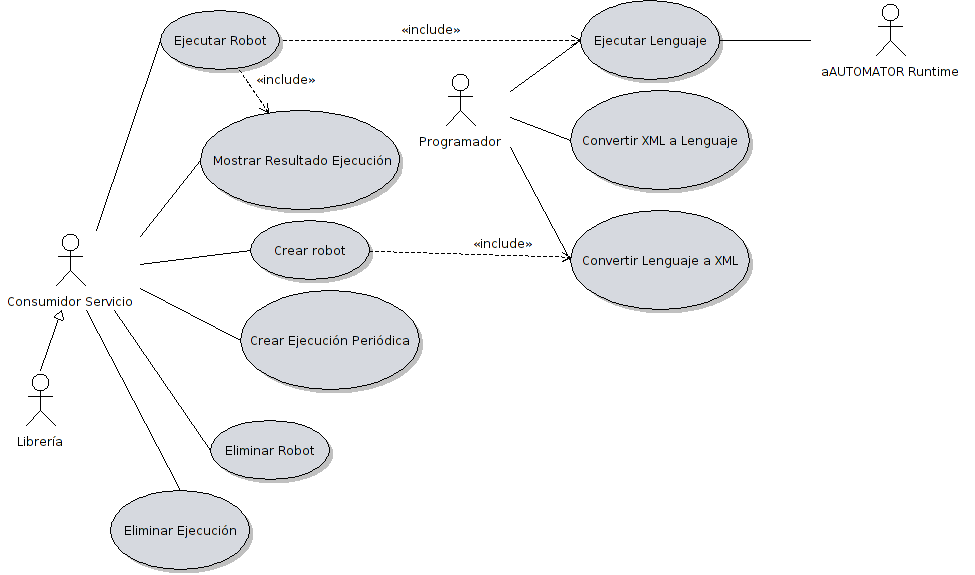
\includegraphics[width=1.4\textwidth]{chapters/technical-manual/diagrams/principal_usecases.violet.png}
\caption{Diagrama Casos Usos principales}\label{casos_uso_principales}
\end{figure}
\end{landscape}

\subsubsection{\large{Caso de uso: Ejecutar Lenguaje}}
\label{ejecutar_lenguaje_caso_uso_minilenguaje}

\begin{tabular}[h]{ p{.3\textwidth } p{.7\textwidth }}

\textbf{Descripción} & El sistema ejecuta el robot especificado en el
lenguaje creado por el proyecto. El lenguaje ha de tener las
características establecidas en \ref{requisitos_lenguaje_robots},
pág.~\pageref{requisitos_lenguaje_robots}.\\[3mm]

\textbf{Actores} & Programador, aAUTOMATOR \emph{Runtime}.\\[3mm]

\textbf{Precondiciones} & - \\[3mm]

\textbf{Postcondiciones} & - \\[3mm]

\textbf{Flujo principal} & \begin{enumerate}[leftmargin=1em,topsep=0pt, partopsep=0pt]
  \item El programador crea o edita un robot en el lenguaje definido
    por el proyecto.
  \item El sistema transforma el lenguaje al XML de
    aAUTOMATOR. [\emph{Excepción A}]
  \item El sistema solicita al aAUTOMATOR \emph{Runtime} que se
    ejecute con un vector de entradas proporcionado por el
    programador. [\emph{Excepción B}]
  \item El sistema muestra el resultado al programador.
\end{enumerate}\\[3mm]

\textbf{Flujos alternativos o Excepciones} &
\begin{enumerate}[label=\Alph*:,leftmargin=1em,topsep=0pt, partopsep=0pt]
\item Lenguaje con sintaxis incorrecta
  \begin{enumerate}[label=\arabic*.,topsep=0pt, partopsep=0pt]
    \item Se muestra al programador el error producido.
  \end{enumerate}
\item Error en ejecución aAUTOMATOR
  \begin{enumerate}[label=\arabic*.,topsep=0pt, partopsep=0pt]
    \item Se muestra al programador el error producido.
  \end{enumerate}
\end{enumerate}\\[3mm]
\end{tabular}

\begin{figure}[bp!]
  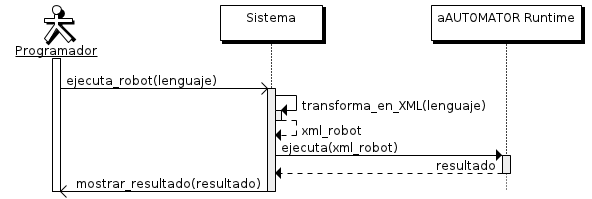
\includegraphics[totalheight=.2\textheight]{chapters/technical-manual/diagrams/sequence/ejecutar_lenguaje.png}
\caption{Ejecutar Lenguaje}\label{ejecutar_lenguaje}
\end{figure}
\clearpage

\subsubsection{\large{Caso de uso: Convertir XML a Lenguaje}}

\begin{tabular}[h]{ p{.3\textwidth } p{.7\textwidth }}

\textbf{Descripción} & Tomar el XML de aAUTOMATOR
~\ref{formato_almacenamiento}, pág.~\pageref{formato_almacenamiento}
y convertirlo en lenguaje. Esto es especialmente útil para la
herramienta visual, permitiendo ver la definición en el lenguaje del
robot que está siendo creado.\\[3mm]

\textbf{Actores} & Programador.\\[3mm]

\textbf{Precondiciones} & - \\[3mm]

\textbf{Postcondiciones} & - \\[3mm]

\textbf{Flujo principal} & \begin{enumerate}[leftmargin=1em,topsep=0pt, partopsep=0pt]
  \item El programador proporciona un XML de aAUTOMATOR válido. [\emph{Excepción A}]
  \item El sistema muestra el lenguaje creado.
\end{enumerate}\\[3mm]

\textbf{Flujos alternativos o Excepciones} &
\begin{enumerate}[label=\Alph*:,leftmargin=1em,topsep=0pt, partopsep=0pt]
\item XML de aAUTOMATOR incorrecto
  \begin{enumerate}[label=\arabic*.,topsep=0pt, partopsep=0pt]
    \item Se muestra al programador el error de formato existente.
  \end{enumerate}
\end{enumerate}\\[3mm]
\end{tabular}

\begin{figure}[bp!]
  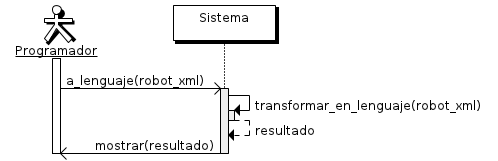
\includegraphics[width=1\textwidth]{chapters/technical-manual/diagrams/sequence/convertir_xml_a_lenguaje.png}
\caption{Convertir XML a Lenguaje}
\end{figure}
\clearpage

\subsubsection{\large{Caso de uso: Convertir Lenguaje a XML}}
\label{convertir_lenguaje_a_xml_caso_uso}
\begin{tabular}[h]{ p{.3\textwidth } p{.7\textwidth }}

\textbf{Descripción} & El sistema convierte el robot especificado en
el lenguaje creado al formato XML soportado por
aAUTOMATOR. Ver~\ref{formato_almacenamiento},
pág.~\pageref{formato_almacenamiento}. \\[3mm]

\textbf{Actores} & Programador.\\[3mm]

\textbf{Precondiciones} & - \\[3mm]

\textbf{Postcondiciones} & - \\[3mm]

\textbf{Flujo principal} & \begin{enumerate}[leftmargin=1em,topsep=0pt, partopsep=0pt]
  \item El programador crea o edita un robot en el lenguaje definido
    por el proyecto.
  \item El sistema transforma el lenguaje al XML de
    aAUTOMATOR. [\emph{Excepción A}]
\end{enumerate}\\[3mm]

\textbf{Flujos alternativos o Excepciones} &
\begin{enumerate}[label=\Alph*:,leftmargin=1em,topsep=0pt,
    partopsep=0pt]
\item Lenguaje con sintaxis incorrecta
  \begin{enumerate}[label=\arabic*.,topsep=0pt, partopsep=0pt]
    \item Se muestra al programador el error producido.
  \end{enumerate}
\end{enumerate}\\[3mm]
\end{tabular}

\begin{figure}[bp!]
  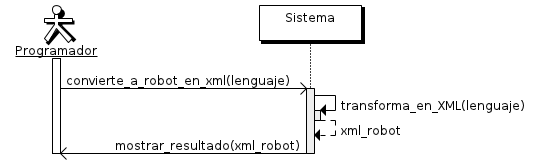
\includegraphics[width=1\textwidth]{chapters/technical-manual/diagrams/sequence/convertir_lenguaje_a_xml.png}
\caption{Convertir Lenguaje a XML}
\end{figure}
\clearpage

\subsubsection{\large{Caso de uso: Mostrar Resultado Ejecución}}
\label{mostrar_resultado_ejecucion_servicio}
\begin{tabular}[h]{ p{.3\textwidth } p{.7\textwidth }}

\textbf{Descripción} & Muestra el resultado de una ejecución. Debe
contener datos como el vector de salida, la fecha en la que se ha
llevado a cabo, el tiempo transcurrido en la ejecución y una
referencia al robot a partir del cual ha sido creada.\\[3mm]

\textbf{Actores} & Consumidor Servicio (p.~ej.: Librería).\\[3mm]

\textbf{Precondiciones} & - \\[3mm]

\textbf{Postcondiciones} & - \\[3mm]

\textbf{Flujo principal} & \begin{enumerate}[leftmargin=1em,topsep=0pt, partopsep=0pt]
  \item El consumidor del servicio accede a una URL que referencia una
    ejecución. [\emph{Excepción A}]
  \item El sistema devuelve información sobre la ejecución.
\end{enumerate}\\[3mm]

\textbf{Flujos alternativos o Excepciones} &
\begin{enumerate}[label=\Alph*:,leftmargin=1em,topsep=0pt, partopsep=0pt]
\item No existe ejecución con ese código
  \begin{enumerate}[label=\arabic*.,topsep=0pt, partopsep=0pt]
    \item Mostrar error indicando que no existe ejecución con ese
      código.
  \end{enumerate}
\end{enumerate}\\[3mm]
\end{tabular}

\begin{figure}[bp!]
  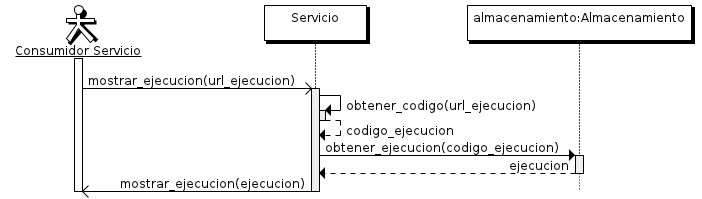
\includegraphics[width=1\textwidth]{chapters/technical-manual/diagrams/sequence/mostrar_resultado_ejecucion.png}
\caption{Mostrar Resultado Ejecución}
\end{figure}
\clearpage

\subsubsection{\large{Caso de uso: Ejecutar Robot}}

\begin{tabular}[h]{ p{.3\textwidth } p{.7\textwidth }}

\textbf{Descripción} & Se indica un robot y un vector de entrada con
el que ejecutarlo. Con esta información se puede realizar una
ejecución del robot en aAUTOMATOR siguiendo
\ref{ejecutar_lenguaje_caso_uso_minilenguaje},
pág.~\pageref{ejecutar_lenguaje_caso_uso_minilenguaje}. Una vez
  finalizada se muestra el resultado al consumidor del servicio
  siguiendo \ref{mostrar_resultado_ejecucion_servicio},
  pág.~\pageref{mostrar_resultado_ejecucion_servicio}\\[3mm]

\textbf{Actores} & Consumidor Servicio (p.~ej.: Librería).\\[3mm]

\textbf{Precondiciones} & - \\[3mm]

\textbf{Postcondiciones} & Existe una nueva ejecución \\[3mm]

\textbf{Flujo principal} & \begin{enumerate}[leftmargin=1em,topsep=0pt, partopsep=0pt]
  \item El Consumidor Servicio indica el código del robot que se
    quiere ejecutar más un vector de entradas. [\emph{Excepción A}]
  \item El robot especificado se ejecuta por aAUTOMATOR
    \emph{Runtime},
    ver~\pageref{ejecutar_lenguaje_caso_uso_minilenguaje}.
    [\emph{Excepción B}]
  \item El resultado obtenido se muestra al Consumidor del
    Servicio. Ver~\ref{mostrar_resultado_ejecucion_servicio}.
\end{enumerate}\\[3mm]

\textbf{Flujos alternativos o Excepciones} &
\begin{enumerate}[label=\Alph*:,leftmargin=1em,topsep=0pt,
    partopsep=0pt]
\item El robot no existe
  \begin{enumerate}[label=\arabic*.,topsep=0pt, partopsep=0pt]
    \item Se deniega la petición indicando la causa.
  \end{enumerate}
\item Error ejecución aAUTOMATOR
  \begin{enumerate}[label=\arabic*.,topsep=0pt, partopsep=0pt]
     \item El resultado mostrado contendrá una descripción del error
       en vez de un resultado convencional.
  \end{enumerate}
\end{enumerate}\\[3mm]
\end{tabular}

\begin{figure}[bp!]
  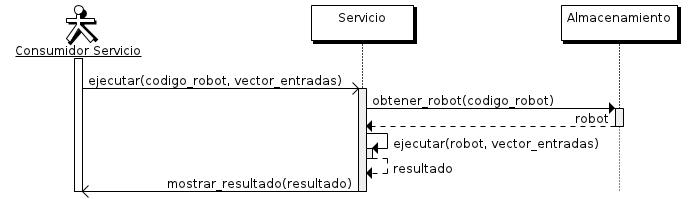
\includegraphics[width=1\textwidth]{chapters/technical-manual/diagrams/sequence/ejecutar_robot.png}
\caption{Ejecutar Robot}
\end{figure}
\clearpage

\subsubsection{\large{Caso de uso: Crear Robot}}

\begin{tabular}[h]{ p{.3\textwidth } p{.7\textwidth }}

\textbf{Descripción} & Crear y almacenar un Robot en el sistema a
partir de un robot tanto en XML como en el lenguaje definido en este
proyecto. \\[3mm]

\textbf{Actores} & Consumidor Servicio (p.~ej.: Librería).\\[3mm]

\textbf{Precondiciones} & - \\[3mm]

\textbf{Postcondiciones} & Se almacena un Robot en el sistema pudiendo
ser referenciado posteriormente. \\[3mm]

\textbf{Flujo principal} & \begin{enumerate}[leftmargin=1em,topsep=0pt, partopsep=0pt]
  \item El \emph{Consumidor Servicio} hace una petición que incluye un robot
    de aAUTOMATOR en XML o en el lenguaje definido en este
    proyecto. [\emph{Excepción A}]
  \item Si el robot no está especificado en XML se convierte al
    mismo. Ver \ref{convertir_lenguaje_a_xml_caso_uso},
    pág.~\pageref{convertir_lenguaje_a_xml_caso_uso}.
  \item Se almacena el robot con la información suministrada.
\end{enumerate}\\[3mm]

\textbf{Flujos alternativos o Excepciones} &
\begin{enumerate}[label=\Alph*:,leftmargin=1em,topsep=0pt, partopsep=0pt]
\item Lenguaje con sintaxis incorrecta
  \begin{enumerate}[label=\arabic*.,topsep=0pt, partopsep=0pt]
    \item Se rechaza la petición indicando el error producido.
  \end{enumerate}
\end{enumerate}\\[3mm]
\end{tabular}

\begin{figure}[bp!]
  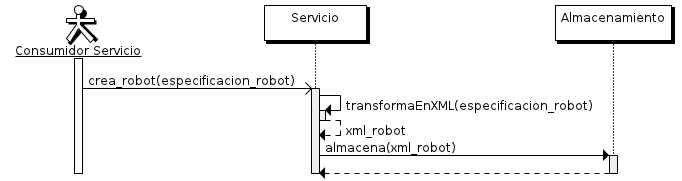
\includegraphics[width=1\textwidth]{chapters/technical-manual/diagrams/sequence/crear_robot.png}
\caption{Crear Robot}
\end{figure}
\clearpage
\subsubsection{\large{Caso de uso: Crear Ejecución Periódica}}

\begin{tabular}[h]{ p{.3\textwidth } p{.7\textwidth }}

\textbf{Descripción} & Crear y almacenar una ejecución periódica a
partir de una referencia a un robot, un periodo de tiempo y un vector
de cadenas de entrada. La ejecución se realizará cada vez que
transcurra el periodo especificado. \\[3mm]

\textbf{Actores} & Consumidor Servicio (p.~ej.: Librería).\\[3mm]

\textbf{Precondiciones} & - \\[3mm]

\textbf{Postcondiciones} & Se realizará la ejecución del robot
referenciado cada vez que transcurra el periodo especificado. El
resultado de la última de estas ejecuciones puede ser mostrado.\\[3mm]

\textbf{Flujo principal} & \begin{enumerate}[leftmargin=1em,topsep=0pt, partopsep=0pt]
  \item El \emph{Consumidor Servicio} hace una petición que referencia
    un robot ya existente, incluye un periodo de tiempo y especifica
    un vector de cadenas de entrada. [\emph{Excepción A}]
  \item Se almacena una ejecución periódica en el sistema de modo que
    se ejecute según el periodo indicado.
\end{enumerate}\\[3mm]

\textbf{Flujos alternativos o Excepciones} &
\begin{enumerate}[label=\Alph*:,leftmargin=1em,topsep=0pt, partopsep=0pt]
\item El periodo es incorrecto.
  \begin{enumerate}[label=\arabic*.,topsep=0pt, partopsep=0pt]
    \item Se deniega la petición indicando la causa.
  \end{enumerate}
\end{enumerate}\\[3mm]
\end{tabular}

\begin{figure}[bp!]
  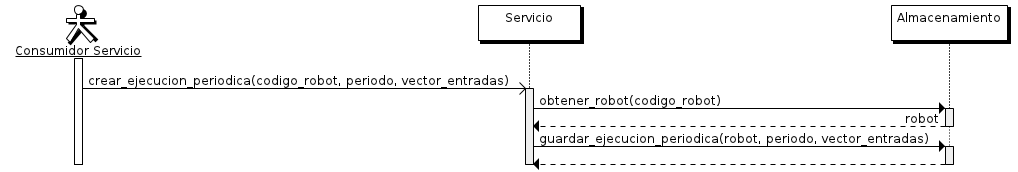
\includegraphics[width=1\textwidth]{chapters/technical-manual/diagrams/sequence/crear_ejecucion_periodica.png}
\caption{Crear Ejecución Periódica}
\end{figure}
\clearpage

\subsubsection{\large{Caso de uso: Eliminar Robot}}

\begin{tabular}[h]{ p{.3\textwidth } p{.7\textwidth }}
\textbf{Descripción} & Elimina un robot existente en el sistema junto
a todos sus datos asociados. \\[3mm]

\textbf{Actores} & Consumidor Servicio (p.~ej.: Librería).\\[3mm]

\textbf{Precondiciones} & - \\[3mm]

\textbf{Postcondiciones} & El robot mas todas sus ejecuciones
asociadas dejan de poder ser referenciados. \\[3mm]

\textbf{Flujo principal} & \begin{enumerate}[leftmargin=1em,topsep=0pt, partopsep=0pt]
  \item El \emph{Consumidor Servicio} hace una petición pidiendo que
    el robot referenciado sea eliminado. [\emph{Excepción A}]
  \item El sistema elimina el robot indicado, junto a las ejecuciones
    asociadas.
\end{enumerate}\\[3mm]

\textbf{Flujos alternativos o Excepciones} &
\begin{enumerate}[label=\Alph*:,leftmargin=1em,topsep=0pt, partopsep=0pt]
\item El Robot no existe.
  \begin{enumerate}[label=\arabic*.,topsep=0pt, partopsep=0pt]
    \item No es necesario hacer nada.
  \end{enumerate}
\end{enumerate}\\[3mm]
\end{tabular}

\begin{figure}[bp!]
  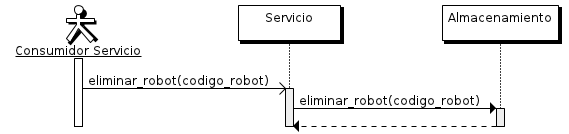
\includegraphics[width=1\textwidth]{chapters/technical-manual/diagrams/sequence/eliminar_robot.png}
\caption{Eliminar Robot}
\end{figure}
\clearpage
\subsubsection{\large{Caso de uso: Eliminar Ejecución}}

\begin{tabular}[h]{ p{.3\textwidth } p{.7\textwidth }}

\textbf{Descripción} &  Elimina una ejecución existente en el sistema. \\[3mm]

\textbf{Actores} & Consumidor Servicio (p.~ej.: Librería).\\[3mm]

\textbf{Precondiciones} & - \\[3mm]

\textbf{Postcondiciones} & La ejecución deja de poder ser referenciada. \\[3mm]

\textbf{Flujo principal} & \begin{enumerate}[leftmargin=1em,topsep=0pt, partopsep=0pt]
  \item El \emph{Consumidor Servicio} hace una petición pidiendo que
    la ejecución referenciada sea eliminada. [\emph{Excepción A}]
  \item El sistema elimina la ejecución indicada.
\end{enumerate}\\[3mm]

\textbf{Flujos alternativos o Excepciones} &
\begin{enumerate}[label=\Alph*:,leftmargin=1em,topsep=0pt, partopsep=0pt]
\item La Ejecución no existe
  \begin{enumerate}[label=\arabic*.,topsep=0pt, partopsep=0pt]
    \item No es necesario hacer nada.
  \end{enumerate}
\end{enumerate}\\[3mm]
\end{tabular}

\begin{figure}[bp!]
  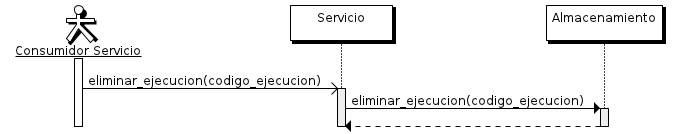
\includegraphics[width=1\textwidth]{chapters/technical-manual/diagrams/sequence/eliminar_ejecucion.png}
\caption{Eliminar Ejecución}
\end{figure}
\clearpage

\subsection{Casos Uso de Aplicación Línea Comandos}
\label{casos_uso_cli_section}
\begin{figure}[p]
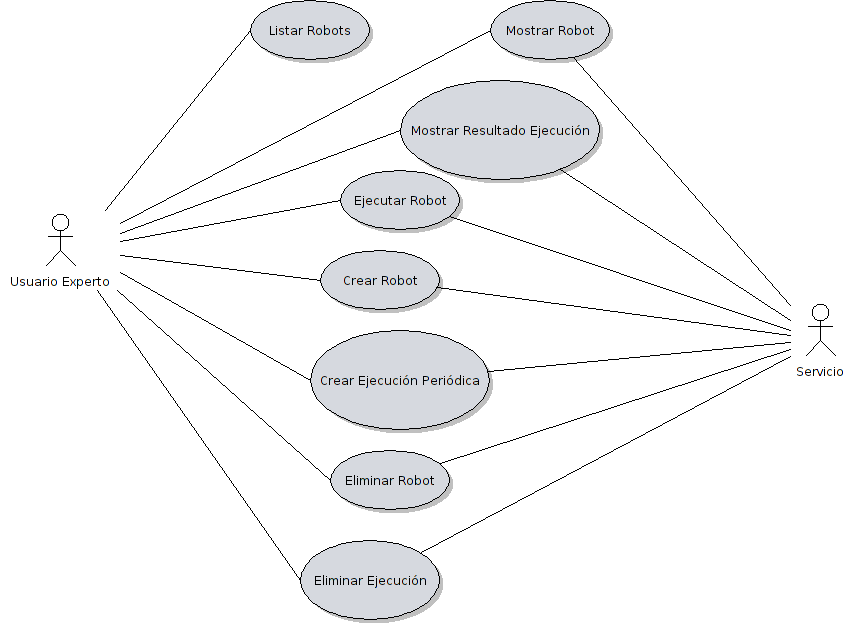
\includegraphics[width=\textwidth]{chapters/technical-manual/diagrams/cli.violet.png}
\caption{Diagrama Casos Usos Línea Comandos}\label{casos_uso_cli}
\end{figure}

\subsubsection{\large{Caso de uso: Listar Robots}}
\label{listar_robots}

\begin{tabular}[h]{ p{.3\textwidth } p{.7\textwidth }}

\textbf{Descripción} & Permite listar los robots creados por un
usuario localmente junto a información asociada. Esto es útil para
facilitar el acceso a los últimos Robots con los que se ha
trabajado.\\[3mm]

\textbf{Actores} & Usuario Experto.\\[3mm]

\textbf{Precondiciones} & - \\[3mm]

\textbf{Postcondiciones} & - \\[3mm]

\textbf{Flujo principal} & \begin{enumerate}[leftmargin=1em,topsep=0pt, partopsep=0pt]
  \item El usuario solicita ver los robots creados desde ese equipo.
  \item El sistema muestra un listado de los robots junto a sus
    ejecuciones asociadas.
\end{enumerate}\\[3mm]

\textbf{Flujos alternativos o Excepciones} &
\end{tabular}

\begin{figure}[bp!]
  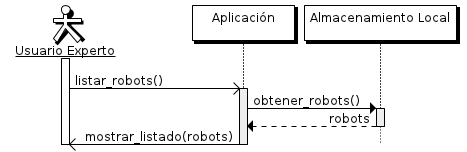
\includegraphics[width=1\textwidth]{chapters/technical-manual/diagrams/sequence/expert_user/listar_robots.png}
\caption{Listar Robots}
\end{figure}
\clearpage
\subsubsection{\large{Caso de uso: Mostrar Robot}}

\begin{tabular}[h]{ p{.3\textwidth } p{.7\textwidth }}

\textbf{Descripción} & Muestra la definición del Robot indicado
accediendo al servicio.\\[3mm]

\textbf{Actores} & Usuario Experto, Servicio.\\[3mm]

\textbf{Precondiciones} & - \\[3mm]

\textbf{Postcondiciones} & - \\[3mm]

\textbf{Flujo principal} & \begin{enumerate}[leftmargin=1em,topsep=0pt, partopsep=0pt]
  \item El usuario indica el código del Robot que quiere mostrar. [\emph{Excepción A}]
  \item Se accede al servicio y se muestra la definición del robot al
    usuario.
\end{enumerate}\\[3mm]

\textbf{Flujos alternativos o Excepciones} &
\begin{enumerate}[label=\Alph*:,leftmargin=1em,topsep=0pt, partopsep=0pt]
\item El robot no existe
  \begin{enumerate}[label=\arabic*.,topsep=0pt, partopsep=0pt]
    \item Se indica al usuario que el robot no existe.
  \end{enumerate}
\end{enumerate}\\[3mm]
\end{tabular}

\begin{figure}[bp!]
  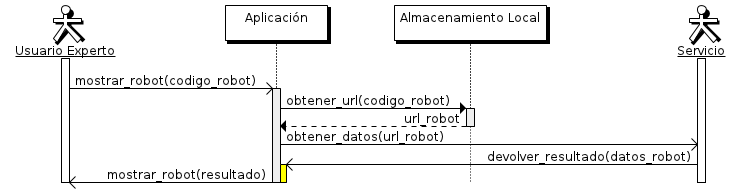
\includegraphics[width=1\textwidth]{chapters/technical-manual/diagrams/sequence/expert_user/mostrar_robot.png}
\caption{Mostrar Robot}
\end{figure}
\clearpage
\subsubsection{\large{Caso de uso: Mostrar Resultado Ejecución}}

\begin{tabular}[h]{ p{.3\textwidth } p{.7\textwidth }}

\textbf{Descripción} & Muestra la definición de la ejecución
especificada accediendo al servicio. \\[3mm]

\textbf{Actores} & Usuario Experto, Servicio.\\[3mm]

\textbf{Precondiciones} & - \\[3mm]

\textbf{Postcondiciones} & - \\[3mm]

\textbf{Flujo principal} & \begin{enumerate}[leftmargin=1em,topsep=0pt, partopsep=0pt]
  \item El usuario indica el código de la Ejecución que quiere mostrar. [\emph{Excepción A}]
  \item La aplicación accede al servicio y se muestran los datos de la
    Ejecución especificada.
\end{enumerate}\\[3mm]

\textbf{Flujos alternativos o Excepciones} &
\begin{enumerate}[label=\Alph*:,leftmargin=1em,topsep=0pt, partopsep=0pt]
\item La Ejecución no existe.
  \begin{enumerate}[label=\arabic*.,topsep=0pt, partopsep=0pt]
    \item Se informa al usuario de la que la ejecución no existe.
  \end{enumerate}
\end{enumerate}\\[3mm]
\end{tabular}

\begin{figure}[bp!]
  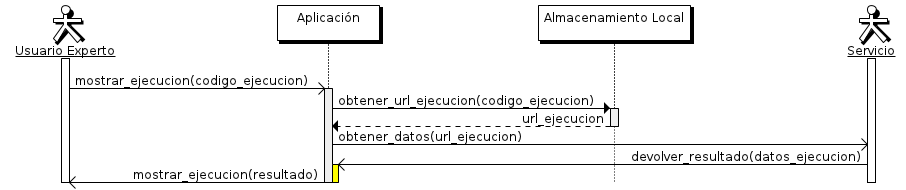
\includegraphics[width=1\textwidth]{chapters/technical-manual/diagrams/sequence/expert_user/mostrar_resultado_ejecucion.png}
\caption{Mostrar Resultado Ejecución}
\end{figure}
\clearpage

\subsubsection{\large{Caso de uso: Ejecutar Robot}}

\begin{tabular}[h]{ p{.3\textwidth } p{.7\textwidth }}

\textbf{Descripción} & Ejecuta el Robot especificado con el vector de
cadenas de entrada especificado. Se comunica con el servicio para
llevarlo a cabo.\\[3mm]

\textbf{Actores} & Usuario Experto, Servicio.\\[3mm]

\textbf{Precondiciones} & - \\[3mm]

\textbf{Postcondiciones} & - \\[3mm]

\textbf{Flujo principal} & \begin{enumerate}[leftmargin=1em,topsep=0pt, partopsep=0pt]
  \item El usuario indica el código del Robot que quiere ejecutar
    junto al vector de cadenas de entrada. [\emph{Excepción A}]
  \item La aplicación accede al servicio y le indica que ha de
    realizar una ejecución con el robot especificado y el vector de
    cadenas de entrada.
\end{enumerate}\\[3mm]

\textbf{Flujos alternativos o Excepciones} &
\begin{enumerate}[label=\Alph*:,leftmargin=1em,topsep=0pt, partopsep=0pt]
\item No existe un Robot con ese código.
  \begin{enumerate}[label=\arabic*.,topsep=0pt, partopsep=0pt]
    \item Se indica al usuario que el robot no existe.
  \end{enumerate}
\end{enumerate}\\[3mm]
\end{tabular}

\begin{figure}[bp!]
  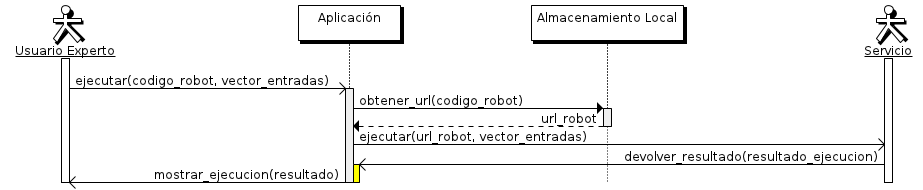
\includegraphics[width=1\textwidth]{chapters/technical-manual/diagrams/sequence/expert_user/ejecutar_robot.png}
\caption{Ejecutar Robot}
\end{figure}
\clearpage
\subsubsection{\large{Caso de uso: Crear Robot}}

\begin{tabular}[h]{ p{.3\textwidth } p{.7\textwidth }}

\textbf{Descripción} & Crea un nuevo Robot en el servicio ya sea a
partir del formato XML o del lenguaje definido en este
proyecto.\\[3mm]

\textbf{Actores} & Usuario Experto, Servicio.\\[3mm]

\textbf{Precondiciones} & - \\[3mm]

\textbf{Postcondiciones} & Un nuevo Robot es creado y almacenado en el
Servicio. El Robot creado aparecerá en el listado.\\[3mm]

\textbf{Flujo principal} & \begin{enumerate}[leftmargin=1em,topsep=0pt, partopsep=0pt]
  \item El usuario proporciona el XML o una instancia del lenguaje
    definido.
  \item El servicio crea un nuevo robot a partir de estos
    datos. [\emph{Excepción A}]
  \item Se guarda la URL del robot creado para que pueda ser accedido
    posteriormente por su código.
\end{enumerate}\\[3mm]

\textbf{Flujos alternativos o Excepciones} &
\begin{enumerate}[label=\Alph*:,leftmargin=1em,topsep=0pt, partopsep=0pt]
\item El robot especificado es incorrecto.
  \begin{enumerate}[label=\arabic*.,topsep=0pt, partopsep=0pt]
    \item Se cancela la petición de creación de Robot y se muestra el
      error al usuario.
  \end{enumerate}
\end{enumerate}\\[3mm]
\end{tabular}

\begin{figure}[bp!]
  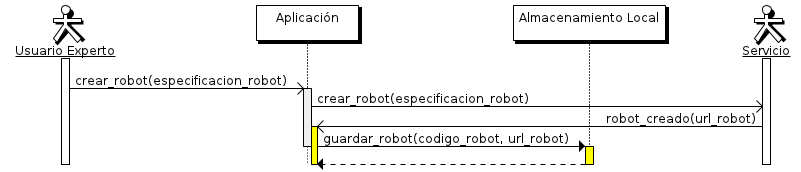
\includegraphics[width=1\textwidth]{chapters/technical-manual/diagrams/sequence/expert_user/crear_robot.png}
\caption{Crear Robot}
\end{figure}
\clearpage
\subsubsection{\large{Caso de uso: Crear Ejecución Periódica}}

\begin{tabular}[h]{ p{.3\textwidth } p{.7\textwidth }}

\textbf{Descripción} & Crea una nueva Ejecución Periódica a partir del
código de un Robot ya existente, un periodo de tiempo y un vector de
cadena de entradas.  La ejecución se realizará cada vez que transcurra
el periodo especificado.\\[3mm]

\textbf{Actores} & Usuario Experto, Servicio.\\[3mm]

\textbf{Precondiciones} & - \\[3mm]

\textbf{Postcondiciones} & Se realizará la ejecución del robot
referenciado en el servicio cada vez que transcurra el periodo
especificado. El resultado de la última de estas ejecuciones puede ser
mostrado. \\[3mm]

\textbf{Flujo principal} & \begin{enumerate}[leftmargin=1em,topsep=0pt, partopsep=0pt]
  \item El usuario indica un el código de un Robot, un periodo de
    tiempo y un vector de cadena de entradas.
  \item El servicio recibe los datos de entrada y crea una ejecución
    periódica. [\emph{Excepción A}]
\end{enumerate}\\[3mm]

\textbf{Flujos alternativos o Excepciones} &
\begin{enumerate}[label=\Alph*:,leftmargin=1em,topsep=0pt, partopsep=0pt]
\item El Robot indicado no existe
  \begin{enumerate}[label=\arabic*.,topsep=0pt, partopsep=0pt]
    \item Se indica la situación al usuario.
  \end{enumerate}
\end{enumerate}\\[3mm]
\end{tabular}

\begin{figure}[bp!]
  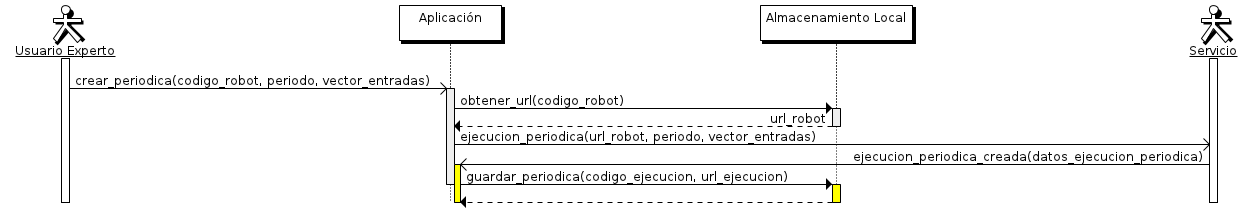
\includegraphics[width=1\textwidth]{chapters/technical-manual/diagrams/sequence/expert_user/crear_ejecucion_periodica.png}
\caption{Crear Ejecución Periódica}
\end{figure}
\clearpage
\subsubsection{\large{Caso de uso: Eliminar Robot}}

\begin{tabular}[h]{ p{.3\textwidth } p{.7\textwidth }}

\textbf{Descripción} & Elimina un robot existente en el sistema junto
a todos sus datos asociados.\\[3mm]

\textbf{Actores} & Usuario Experto, Servicio.\\[3mm]

\textbf{Precondiciones} & - \\[3mm]

\textbf{Postcondiciones} & El robot mas todas sus ejecuciones
asociadas dejan de poder ser referenciados. Tampoco aparecerán en el
listado local Ver \ref{listar_robots},
pág~\pageref{listar_robots}.\\[3mm]

\textbf{Flujo principal} & \begin{enumerate}[leftmargin=1em,topsep=0pt, partopsep=0pt]
  \item El usuario indica el código del Robot que desea eliminar.
  \item Se elimina el Robot indicado, junto a las ejecuciones
    asociadas del almacenamiento local.
  \item El servicio elimina el Robot indicado, junto a las ejecuciones
    asociadas. [\emph{Excepción A}]
\end{enumerate}\\[3mm]

\textbf{Flujos alternativos o Excepciones} &
\begin{enumerate}[label=\Alph*:,leftmargin=1em,topsep=0pt, partopsep=0pt]
\item El Robot no existe.
  \begin{enumerate}[label=\arabic*.,topsep=0pt, partopsep=0pt]
    \item No es necesario hacer nada.
  \end{enumerate}
\end{enumerate}\\[3mm]
\end{tabular}

\begin{figure}[bp!]
  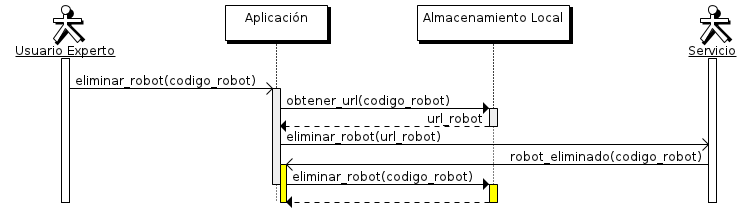
\includegraphics[width=1\textwidth]{chapters/technical-manual/diagrams/sequence/expert_user/eliminar_robot.png}
\caption{Eliminar Robot}
\end{figure}
\clearpage
\subsubsection{\large{Caso de uso: Eliminar Ejecución}}

\begin{tabular}[h]{ p{.3\textwidth } p{.7\textwidth }}

\textbf{Descripción} &  Elimina una ejecución del servicio y
localmente, de modo que no pueda volver a ser accesible. \\[3mm]

\textbf{Actores} & Usuario Experto, Servicio.\\[3mm]

\textbf{Precondiciones} & - \\[3mm]

\textbf{Postcondiciones} & La Ejecución indicada deja de poder ser
referenciada. Tampoco aparecerán en el listado local Ver
\ref{listar_robots}, pág~\pageref{listar_robots}. \\[3mm]

\textbf{Flujo principal} & \begin{enumerate}[leftmargin=1em,topsep=0pt, partopsep=0pt]
  \item El usuario indica el código de la Ejecución que desea
    eliminar.
  \item Se elimina del almacenamiento local la Ejecución indicada.
  \item El servicio elimina la ejecución indicada. [\emph{Excepción A}]
\end{enumerate}\\[3mm]

\textbf{Flujos alternativos o Excepciones} &
\begin{enumerate}[label=\Alph*:,leftmargin=1em,topsep=0pt, partopsep=0pt]
\item La Ejecución no existe.
  \begin{enumerate}[label=\arabic*.,topsep=0pt, partopsep=0pt]
    \item No es necesario hacer nada.
  \end{enumerate}
\end{enumerate}\\[3mm]
\end{tabular}

\begin{figure}[bp!]
  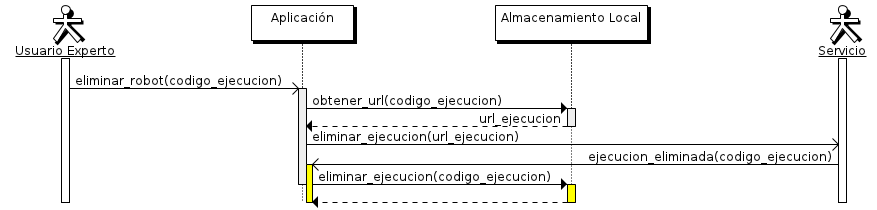
\includegraphics[width=1\textwidth]{chapters/technical-manual/diagrams/sequence/expert_user/eliminar_ejecucion.png}
\caption{Eliminar Ejecución}
\end{figure}
\clearpage


\section{Diseño}
En esta sección se detalla el diseño del sistema. Primero haremos una
descripción y justificación de las grandes decisiones arquitectónicas
tomadas, para luego hacer una descripción más detallada del sistema
entregado.

\subsection{Minilenguaje como DSL interna}
Finalmente la DSL se ha implementado por medio de una DSL~interna en
JRuby. Discutiremos las características de las DSL~internas y las
DSL~externas, así como la razón para elegir JRuby.
\subsubsection{DSL internas}

Las DSL internas se desarrollan utiizando las facilidades ofrecidas
por el lenguaje de programación en el que se realiza. Esto colleva que
estés limitado por las las características de dicho lenguaje. A medio
camino entre librería y DSL interna se encuentran las llamadas
\emph{fluent interfaces}. Muchas veces es difícil distinguir una
\emph{fluent interface} de una DSL interna; teniendo las DSL internas
mayores características de un lenguaje.

\subsubsection{DSL externas}

Con las DSL internas siempre estás limitado en cierta medida por la
sintaxis del lenguaje anfitrión. Las DSL externas proporcionan, sin
embargo, libertad absoluta. La DSL externa opera en texto, aplicando
un proceso de parseado. Las técnicas para parsear el texto de entrada
son las mismas que las utilizadas para implementar un lenguaje de
programación. Conviene recordar que lo que distingue a una DSL de un
lenguaje de programación es que está orientada a un campo específico.

En el caso de decidir realizar una DSL externa se podría elegir entre
varias técnicas para realizar el parseado:
\begin{description}
\item[Recursive Descent Parser\footnote{Analizador sintáctico
    descendente recursivo}]: Es una forma de traducir un
  \emph{top-down} parser, traduciendo cada símbolo no terminal a una
  función.
\item[Parser Combinator]: Se trata de una variante de lo anterior en
  el que se utilizan combinadores, funciones que aceptan otras
  funciones que representan símbolos no terminales.
\item[Generador Parsers]: Se trata de librerías que reciben una
  gramática en BNF\footnote{Backus-Naus Form} y emiten código para
  crear un parser de un tipo específico. Unas de las más comunes en
  el mundo Java son ANTLR y JavaCC.
\end{description}

\subsubsection{¿Por qué DSL interna?}

Una ventaja de una DSL interna frente a una DSL externa es que en
teoría tienen un coste de desarrollo inferior ya que se utilizan
herramientas con las que el programador ya esta familiarizado. Por
otro lado muchas veces las DSL internas descansan en características
pocos conocidas de los lenguajes anfitriones.

Por otro lado la DSL interna estará limitada por la sintaxis del
lenguaje anfitrión y esto puede limitar su expresividad. Una ventaja
de las DSL internas, sin embargo, es que permiten el uso del lenguaje
anfitrión para exponer estructuras de control, aritmética, etc.

Finalmente hemos optado por desarrollar una DSL interna ya que creímos
que la expresividad de Ruby era suficiente para nuestros
propositos. Para confirmarlo creamos un prototipo de la DSL
interna. Consideramos el resultado suficientemente expresivo por lo
que desechamos la posibilidad de desarrollar una DSL externa. A partir
de este prototipo se ha desarollado el resultado final.

\subsubsection{Ruby y JRuby}
Ruby es una buena opción para realizar DSL internas porque es un
lenguaje que gracias a su sintaxis flexible y sus capacidades de
metaprogramación.
\subsubsection{Sintaxis}
\subsubsection{Ejemplos}

\subsubsection{Inyección código malicioso}
Se ha empleado una sandbox, Java Security Architecture, \ldots{}
\subsubsection{Timeouts}
\subsubsection{Manipulación estado intérprete}
\label{interpreter_state_manipulation}

\subsection{Servicio sigue estilo arquitectónico REST}
REST\footnote{\emph{Representational state transfer}} es un estilo de
arquitectura software empleado en sistemas distribuidos como la
\emph{World Wide Web}, de ahora en adelante \emph{WWW}.

REST fue desarrollado por Roy Fielding entre otros al mismo tiempo que
se desarrollaba la versión 1.1 del protocolo HTTP. Aun así REST se
puede emplear con otros protocolos si proporcionan mecanismos
adecuados para la transferencia de representación.

El objetivo de la WWW era constituir un espacio común de información
en el que máquinas y usuarios se puedan comunicar.  Los usuarios de
este sistema estarían por todo el mundo, en varias universidades e
institutos de investigación conectados a través de Internet. Las
máquinas así conectadas serían de carácter heterogéneo, haciendo
necesario, con una gran variedad de sistemas operativos y formatos. La
información a distribuir iba desde datos de investigación hasta
listados telefónicos. El reto era proporcionar un un sistema que
proporcionase una interfaz consistente y universal a todo esta
información estructurada, disponible en el mayor número de plataformas
posibles y capaz de ser aumentada según nuevos usuarios y
organizaciones se unieran al proyecto.

Como la publicación de información en la WWW era de carácter
voluntario era necesario que las barreras de entrada fueran bajas. Se
eligió \emph{hypermedia} como la interfaz de usuario dada su
simplicidad y generalidad. La misma interfaz puede ser usada
independientemente de la fuente de información. La flexibilidad de los
enlaces permite estructurar sin límites y la manipulación directa de
estos enlaces permite guiar al usuario dentro de la aplicación. Como a
menudo la información dentro de grandes bases de datos es más fácil de
acceder a través de una búsqueda, WWW también ofrecía la posibilidad
de realizar consultas, respondiendo con hypermedia a los datos
introducidos por el usuario.

Hypermedia distribuida implica que la información pueda estar
almacenada en máquinas remotas. Esto conlleva la transferencia de
grandes cantidades de datos desde el lugar de almacenamiento al lugar
de uso. Para la usabilidad de la hypermedia es básico que la latencia
percibida por parte del usuario sea mínima. Por tanto hay que
minimizar las interacciones con la red.

También es importante que la no disponibilidad de parte del sistema,
no impida a los autores crear contenido de manera local. El lenguaje
de \emph{hipertexto} creado debe de ser sencillo y fácil de crear con
las herramientas existentes.

Otro factor importante es que el protocolo está basado en texto. Esto
facilita la vida de los desarrolladores de aplicaciones, ya que
permite observar y probar el protocolo de una manera directa y
sencilla.

Mientras que la simplicidad facilita la adopción del sistema inicial,
la extensibilidad nos permite mejorar el sistema inicial. Un sistema
con objetivos a largo plazo debe de tener mecanismos para ser
modificado.

Así mismo, el sistema esta orientado a ser desplegado en
Internet. Esto significa que el sistema va a ser usado por diferentes
organizaciones con diferentes objetivos. Normalmente los sistemas de
información son controlados por una única organización. Pero en el
caso de la WWW los componentes deben funcionar a pesar de cargas no
anticipadas, datos incorrectos o intencionadamente dañinos, etc. La
escala global conlleva que los clientes no pueden tener conocimiento
de todos los servidores, los servidores no deberían retener estado a
través de varias peticiones. Hypermedia no puede mantener una lista de
páginas que apuntan a un elemento, ya que el número de enlaces puede
ser muy elevado e impredecible.

Dado que la WWW no va a ser controlado por una única organización,
nuevas versiones no se desplegarán homogéneamente. Por tanto,
diferentes versiones de los elementos deben de poder coexistir. Cada
componente debe suponer que nuevas versiones se van a añadir.
Versiones antiguas de un componente deben de ser identificadas de modo
que no interfieran en el funcionamiento de elementos más modernos.

En este contexto, cuando la WWW se empezó a hacer más popular al
principio de los 90 se encontraron numerosas limitaciones a la primera
versión del protocolo HTTP. Las nuevas formas de uso presentaban un
reto para la infraestructura de Internet de aquel momento. Esto
presentaba la necesidad de evolucionar el protocolo HTTP de modo que
fuera mas escalable. ¿Pero que principios usar para guiar su evolución?

La WWW inicial carecía de una arquitectura bien definida. Ante la
existencia de numerosas y a veces contradictorias propuestas para los
diferentes protocolos que forman la WWW, era necesario tener un estilo
arquitectónico. El estilo arquitectónico define una serie de
restricciones; las propuestas han de ser evaluadas contra estas
restricciones buscando posibles conflictos.

Ante esta situación surge el estilo arquitectónico REST con un
especial énfasis en la escalabilidad de la interacción entre
componentes, generalidad de las interfaces, despliegue independiente
de componentes y componentes intermedios para reducir latencia.

REST se define a través de una serie sucesiva de restricciones que los
elementos de la arquitectura deben seguir. REST es, además, un sistema
híbrido derivado de varios estilos arquitectónicos existentes:

\begin{description}

\item[Cliente-Servidor.] La primera restricción es que el sistema debe
  de ser cliente servidor. La separación de intereses es el principio
  detrás de la separación cliente servidor. Separando los
  requerimientos de la interfaz de usuario de los de almacenamiento de
  datos se mejora la portabilidad de la interfaz de usuario y se
  mejora la escabilidad al simplificar los componentes de servidor. En
  el caso de la WwW, esto permite a los diferentes componentes
  evolucionar independientemente.

\item[Sin Estado.] La comunicación entre un cliente y un servidor debe
  de ser sin estado. Esto significa que cada petición del cliente debe
  contener toda la información necesaria para ser procesada, sin
  beneficiarse de contexto adicional almacenado en el servidor. Por
  tanto estado de la sesión debe de ser almacenado en el cliente.

  Esta restricción induce las propiedades de visibiliad, fiabilidad y
  escalabilidad. La visibilidad es mejorada porque un sistema de
  monitorización no tiene que mirar más allá de una única petición
  para determinar la naturaleza de la petición. La fiabilidad mejora
  porque facilita el proceso de recuperarse de fallos transitorios. La
  escalabilidad mejora porque no tener que almacenar estado entre
  peticiones, permite al servidor liberar recursos de manera rápida y
  simplifica la implementación.

  La desventaja de un protocolo sin estado es que el rendimiento de la
  red puede reducirse al tener que transmitir más datos repetidos, ya
  que no se puede mantener en el servidor un contexto
  compartido. Aparte dejar el estado en el cliente, reduce el control
  del servidor sobre el comportamiento consistente de la aplicación,
  ya que la aplicación depende de la implementación correcta del
  comportamiento por los clientes a lo largo de diferentes versiones.

\item[Caché.] Para mejorar la eficiencia de la red, se añaden
  restricciones de caché. Se requiere que los datos dentro de una
  respuesta sean marcados como cacheables o no cacheables. Si una
  respuesta es cacheable, se permite que la caché de un cliente
  reutilice esa respuesta para peticiones posteriores.

  La ventaja fundamental de una caché es que permite eliminar completa
  o parcialmente algunas interacciones, aumentando la eficiencia, la
  escalabilidad y el rendimiento percibido por el usuario al reducir
  la latencia. El inconveniente es que una caché puede reducir la
  fiabilidad, si los datos obtenido de la caché difieren
  considerablemente de los que se obtendrían en una nueva petición.

  Las restricciones presentadas hasta ahora son las que definieron el
  estado inicial de la arquitectura de la WWW.

\item[Interfaz Uniforme.] Esta es la característica principal que
  distingue REST de otros estilos arquitecturales. Al aplicar el
  principio de la generalidad a la interfaz del componente, la
  arquitectura global es simplificada y la visibilidad de las
  interacciones es mejorada. Los servicios ofrecidos están
  desacoplados de las implementaciones, lo que facilita la evolución
  independiente de los mismos. El inconveniente es que una interfaz
  uniforme reduce la eficiencia, ya que la información es transmitida
  en un formato estandarizado en vez de uno específico para la
  aplicación. La interfaz uniforme definida por REST esta diseñada
  para ser eficiente en el caso de transferencias de Hypermedia de
  grano grueso, el caso más típico en la WWW.

  Cuando un enlace es seleccionado, la información necesita ser
  llevada desde el lugar de almacenamiento hasta la localización donde
  va a ser usado. Esto es a diferencia de otros paradigmas
  distribuidos, en los que es muchas más veces más sencillo llevar el
  agente procesador a los datos. Para poder llevar a cabo esta
  transferencia, se transfiere una \emph{representación} del recurso
  en un formato correspondiente a algún tipo estándar. El formato se
  selecciona dinámicamente basado en las características y los deseos
  del cliente y la naturaleza del recurso. Si la representación es el
  mismo formato que el recurso o es derivada de la original, permanece
  oculto tras la interfaz. El formato de la representación es
  conocido como tipo MIME\cite{MIME}. Una representación puede ser
  incluida y procesada por el destinatario en acorde a los datos de
  control del mensaje y la naturaleza del tipo de datos.

  En REST otra abstracción clave a la hora de ofrecer una interfaz
  uniforme son los recursos. Cualquier información que se puede
  nombrar puede ser un recurso: una imagen, un documento, un servicio,
  una colección de recursos, un objeto físico, etc. Cualquier concepto
  que pueda ser referido mediante un enlace de hypertexto es un
  recurso. Un recurso es un conjunto de entidades que en un momento
  dado son equivalentes entre si. Estas entidades son representaciones
  del recurso. Algunos recursos son estáticos, una vez creados no
  varían. Otros son altamente variables y a lo largo del tiempo pasan
  a tener representaciones diferentes. Esta definición abstracta de un
  recurso, permite abarcar numerosas fuentes de información empleando
  la misma interfaz basada en recursos. En la WWW los recursos son
  referenciados por medio de las URI\footnote{\emph{Uniform Resource
      Identifiers}}, combinación de las URL\footnote{\emph{Uniform
      Resource Locator}} y las URN\footnote{\emph{Uniform Resource
      Names}}.

  Podemos ver que cada servidor en la WWW ofrece una interfaz
  abstracta para acceder a los recursos y transferirlos. Cada recurso
  puede ser manipulado con una serie de verbos predefinidos: GET,
  POST, PUT y DELETE. Por lo tanto un servicio REST define un espacio
  de nombres por medio de recursos que pueden ser operados por medio
  de una interfaz genérica basada en los verbos HTTP más tipos
  estándar MIME. Esta serie de recursos definidos por un servicio han
  de tener una semántica clara. La idea es que los nombres de los
  recursos permanezcan más o menos fijos, mientras que las
  representaciones pueden variar.

\item[Sistema en Capas.] Esta restricción mejora el comportamiento para
  requisitos de escalabilidad a nivel de Internet. Esta restricción
  permite a una arquitectura estar compuesta por capas jerárquicas de
  modo que cada capa solo pueda ver más allá de la capa con la que
  están interaccionando. Limitando la visibilidad a la capa inmediata,
  reducimos la complejidad global y promovemos independencia con
  respecto a las otras capas. Las capas se pueden usar para encapsular
  servicios desfasados y para proteger nuevos servicios de clientes
  desfasados, simplificando los componentes al mover funcionalidad
  raramente usada a un intermediario. Los intermediarios también
  pueden ser usados para aumentar la escalabilidad al permitir el uso
  de reparto de carga de un servicio a través de múltiples redes y
  nodos.

\item[Código bajo Demanda.] REST permite que la funcionalidad de los
  clientes pueda ser extendida, descargando y ejecutando código en
  forma de applets y scripts. Esto simplifica los clientes al reducir
  el número de características que tienen que estar
  preinstaladas. Permitir nuevas características a posteriori mejora
  la extensibilidad del sistema.
\end{description}

Una vez hemos descrito REST veamos que nos aporta en relación a DARE y
porque se ha decidido escogerlo.

Consideramos que REST es más práctico. No conlleva la carga conceptual
de, por ejemplo SOAP\cite{SOAP}. Como la WWW está basada en los
conceptos de REST, todos los programadores están familiarizados con
ellos. Mientras es cierto que el soporte de SOAP es extenso y suelen
existir herramientas para facilitar su uso, en muchas plataformas no
es una opción. Por ejemplo, si queremos crear una aplicación web que
acceda al servicio, como es el caso de una de las posibles
ampliaciones de este proyecto. Ver~\ref{MASHUP_REF} en
pág.~\pageref{MASHUP_REF}.

Además REST nos facilita proporcionar diferentes representaciones de
los recursos definidos. Por ejemplo, nos ha facilitado proporcionar
las respuestas tanto en XML como en JSON. Esto es SOAP habría de
realizarse de manera completamente manual.

El hecho de que REST nos obligue a ofrecer un servicio sin estado,
facilita la escalabilidad del mismo en gran manera. Nos permite
introducir un balanceador de carga o proxy inverso. El balanceador de
carga repartirá las peticiones recibidas entre todos los nodos
disponibles. Si se añade un nodo, éste es capaz de empezar a atender
peticiones inmediatamente, ya que no hay un contexto asociado a las
peticiones anteriores. Además nos ayuda a mantener un servicio
altamente fiable. Si uno de los nodos falla, la petición se puede
enviar a cualquiera de los otros nodos, permitiendo que el servicio
siga funcionando. No hacen falta por tanto, complicados mecanismos de
\emph{failover}.

Al usar REST podemos emplear el soporte del protocolo HTTP para
cachear resultados. Esto nos permite evitar transferencias
innecesarias, ahorrando ancho de banda y reduciendo la
latencia. Consideramos que está es una de las claves para obtener un
alto rendimiento en situaciones en las que varios Robots están siendo
accedidos continuamente.

Así mismo, consideramos que una API REST es más fácil de evolucionar y
menos frágil que una equivalente en SOAP. HTTP incorpora mecanismos
para negociar las respuestas dadas, facilitando la coexistencia de
diversas versiones de clientes. En SOAP los nuevos clientes tendrían
que utilizar métodos con nombres distintos o habría que desfasar las
versiones antiguas de los clientes inmediatamente.


\subsubsection{JAX-RS\cite{JAXRS}}

Como hemos explicado la WWW se basa en REST como estilo
arquitectónico. Sería perfectamente viable implementar el servicio
utilizando algún framework o tecnología web típica: CGI, PHP,
Servlets, Struts, Ruby on Rails, etc. Aun así, la mayoría de los
frameworks no fomentan el seguimiento de los principios REST de una
manera rigurosa.

Al final hemos decidido usar el framework JAX-RS. No se trata de una
librería en concreto, sino de una especificación. Ha sido diseñada con
el propósito de crear aplicaciones web siguiendo los principios
REST. El objetivo de la especificación es crear una API de alto nivel,
con un estilo declarativo usando anotaciones.

Hemos considerado que su funcionamiento era adecuado para nuestras
necesidades. Para las necesidades de este proyecto se muestra como una
buena opción. Además tiene una parte de cliente lo que facilitaría la
creación de la librería para la parte Java.

Existen varias implementaciones de esta API. Nos hemos decantado por
la implementación de referencia, Jersey\cite{JERSEY}.

\subsection{MongoDB como Sistema Almacenamiento}
\subsubsection{Bases de datos relacionales y NoSQL}

NoSQL es un conjunto de tipos de bases de datos que difieren del
modelo clásico de RDBMS\footnote{\emph{Relational Database Management
    System}}. La característica más común es que no utilizan SQL como
su lenguaje de consulta. Estos sistemas de almacenamiento de datos no
siempre requieren esquemas de datos fijos, no suelen soportar
operaciones join, no suelen cumplir todas las características
ACID\footnote{\emph{atomiticy, consistency, isolation, durability}} y
suelen estar especialmente pensadas para escalar horizontalmente.

Como se puede observar NoSQL es un término muy amplio, más
caracterizado por lo que no es, que por lo que es. Es más útil hablar
de una categoría en concreto de bases de datos NoSQL. Así podemos
hablar de bases de datos clave-valor, bases de datos orientadas a
documentos y bases de datos orientadas a grafos.

\begin{description}
\item[Clave-valor:] Este tipo tiene un modelo de datos muy
  sencillo. No requieren un esquema fijo como las RDBMS. Gracias a
  este modelo sencillo de datos suelen escalar muy bien
  horizontalmente. Sólo permiten hacer consultas a través de las
  claves.

\item[Documental:] Están basadas en la noción de
  documento. Generalmente asumen que todos los documentos almacenados
  están en un mismo formato: XML, JSON, BSON, etc. Cada documento
  sería similar a una fila en una base de datos relacional, pero su
  estructura es mucho menos rígida, no han de seguir un esquema
  fijo. La diferencia fundamental con respecto a las bases de datos
  clave-valor es que proporcionan un mecanismo de consulta basado en
  los contenidos de los documentos.

\item[Orientada a Grafos:] Utilizan nodos, aristas y propiedades para
  representar y almacenar datos. Sus estructuras de datos son
  similares a las presentes en lenguajes OOP\footnote{\emph{Object
      Oriented Programming}}, permitiendo un mapeo más
  directo. Permiten realizar de manera sencilla consultas basadas en
  grafos, como, por ejemplo, calcular la distancia mínima entre dos
  nodos. El acceso a los datos y nodos asociados a un nodo en concreto
  es más rápido que en una RDBMS. Por contra, las bases de datos
  relacionales son más rápidas realizando la misma operación contra
  una gran cantidad de datos.

\item[Orientada a Objetos:] La información es representada como
  objetos, en el sentido de OOP. Suelen integrarse en el lenguaje OOP
  usado, utilizando el lenguaje y la base de datos las mismas
  definiciones de tipos. Permiten almacenar los objetos usados
  directamente. Obtener un objeto con muchos datos asociados es
  generalmente más rápido que en un RDBMS.

\item[Orientadas a columnas:] En vez de almacenar los datos de una
  fila de manera contigua, almacena los datos de cada columna o un
  conjunto pequeño de columnas de manera contigua. Esto permite
  aplicar algoritmos de comprensión en los datos de cada columna. Las
  bases de datos de este tipo que siguen el modelo
  \emph{BigTable}\cite{BIG-TABLE} de Google se pueden considerar como un mapa
  ordenado multidimensional y distribuido. Están orientadas a
  almacenar cantidades masivas de datos de manera distribuida. Este
  tipo de base de datos suelen estar pensadas para realizar consultas
  y ser modificadas mediante trabajos Map-Reduce\cite{MAP-REDUCE}.

\end{description}

Aunque DARE se podría haber desarrollado en cualquier categoría,
creemos que el tipo de base de datos más adecuado es una base de datos
orientada a documentos. Una base de datos relacional podría haber
servido, pero el esquema de datos habría supuesto una definición muy
rígida de los datos. Esto nos dificultaría la evolución de los datos
en tiempo de desarrollo y en un futuro. Una base de datos orientada a
documentos nos ofrece la posibilidad de guardar los Robots, los
resultados de ejecuciones, las ejecuciones periódicas y los datos
necesarios de manera directa y sencilla. La operación más típica sera
obtener una de estas entidades por clave, con lo cual una base de
datos clave-valor parece ser una buena opción. El problema es que otro
tipo de consultas podrían ser necesarias, por lo que preferimos la
flexibilidad extra que nos proporcionan las bases de datos orientadas
a documentos.

Aun así, hay muchos factores a considerar, como escalabilidad y
facilidad de uso, asi que emplear un RDBMS sigue siendo una opción.

\subsubsection{Opciones valoradas}
\begin{description}

\item[MySQL:] MySQL es un RDBMS ampliamente usado en aplicaciones
  web. Ha demostrado una gran madurez. Ha demostrado ser escalable
  utilizando técnicas como sharding\cite{SHARDING} y replicación
  \emph{master-slave}\cite{MASTER-SLAVE}. Aunque inicialmente MySQL
  carecía de numerosas características propias de un RDBMS (integridad
  referencial, transacciones, triggers, etc.), con el paso del tiempo
  las ha incorporado. Otra ventaja es la madurez y familiaridad con el
  modelo relacional (emplea SQL).
\item[PostgreSQL:] Prácticamente lo mismo dicho sobre MySQL se puede
  aplicar a PostgreSQL. Ambas serían soluciones completamente válidas
  para el problema. PostgreSQL tradicionalmente ha soportado más
  características típicas de un RDBMS pero hoy en día tienen unas
  características bastante parejas. Por otro lado PostgreSQL no
  soportaba replicación, pero las últimas versiones si la soportan. Se
  podría decir que la elección entre PostgreSQL y MySQL es altamente
  subjetiva. En mi caso me decantaría por PostgreSQL por tener, a mi
  juicio, una mayor calidad interna y por su modelo de
  desarrollo. Ambos productos son Software Libre, pero MySQL está
  esponsorizado por una única compañía (Oracle). Por contra,
  PostgreSQL no está controlado por una única compañía.
\item[BerkeleyDB:] Se trata de una base de datos embebida
  clave-valor. Soporta bases de datos de gran tamaño y los valores
  almacenados no tienen un esquema fijo. Soporta algunas
  características avanzadas como transacciones, locking y
  replicación. Se trata de una opción valida aunque su modelo de datos
  no sea tan conveniente como un RDBMS o una base de datos orientada a
  documentos.
\item[Voldemort:] Es una base de datos clave-valor y se puede
  considerar una tabla hash persistente, grande, distribuida y
  tolerante a fallos. Su modelo de datos es muy sencillo, pero es muy
  fácil de escalar entre numerosos nodos. Tanto las lecturas y las
  escrituras se pueden escalar horizontalmente. Utiliza una técnica
  mixta de particionamiento y replicación. Cada nodo es independiente,
  es decir, no existe un único punto de error\footnote{Más conocido
    como \emph{single point of failure}.}.
\item[HBase:] Es una base de datos inicialmente basada en la
  arquitectura de \emph{BigTable} de Google. Tiene un modelo de datos
  basado en agrupación de columnas. Se suele utilizar conjuntamente
  con Hadoop\cite{HADOOP} y no directamente, pero en las últimas
  versiones su rendimiento en cuanto a acceso directo ha mejorado. Un
  problema con HBase es que no se adapta bien a ser ejecutado en un
  único nodo. Esto es un problema ya que DARE ha de tener requisitos
  de hardware modestos cuando el número de usuarios es escaso.
\item[Cassandra:] Es una base de datos que aglutina características
  tanto de Voldermort, como HBase. Su modelo de datos es similar al de
  HBase, pero sus características en cuanto a escalabilidad son
  similares a Voldemort. Carece de un único punto de error. Como
  característica a destacar ofrece la posibilidad de ajustar la
  consistencia requerida en cada operación. Sobre Cassandra podemos
  decir que ofrecería una gran escalabilidad pero su administración y
  conceptos son relativamente complejos.
\end{description}

\subsubsection{MongoDB}
\label{ELECCION-MONGO}

Finalmente hemos optado por utilizar \emph{MongoDB}. Su modelo de
datos orientado a documentos nos ofrece una gran velocidad de
desarrollo. Los documentos son guardados y obtenidos como JSON, lo que
facilita el desarrollo web. Podríamos decir que de todas las bases de
datos mencionadas anteriormente es la que nos ofrece una mayor
velocidad de desarrollo. Una característica que hemos valorado
especialmente es que nos permite hacer consultas arbitrarias
optimizadas por índices.

En cuanto a la administración es relativamente sencilla, aunque aquí
podríamos echar algo en falta la madurez de MySQL y PostgreSQL. Además
cuenta con mecanismos necesarios para escalar la base de datos en el
caso de que fuera necesario. En cuanto a escalabilidad no consta de
las facilidades de Cassandra y Voldemort, pero ofrece mecanismos como
\emph{replica sets} y \emph{sharding}.

\begin{description}
\item[Replica Sets:] Son una forma de replicación asíncrona. Un
  \emph{replica set} contiene dos o más nodos que son copias de cada
  uno. De este conjunto se elige un nodo que se considera el
  primario. Las escrituras se dirigen a este nodo primario. Las
  lecturas se pueden dirigir a cualquier nodo del \emph{replica
    set}. Este diseño nos permite obtener redundancia de datos,
  obteniendo una alta disponibilidad. En el caso de que un nodo
  fallase los restantes nodos pueden seguir funcionando. La carga de
  lecturas es distribuida entre todos los nodos, lo que puede ayudar
  mucho en la escalabilidad del sistema. Ver~\ref{replica-sets}
  en pág.~\pageref{replica-sets}.
  \begin{figure}[hbp]
    \begin{center}
      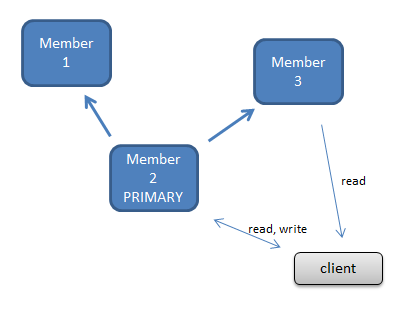
\includegraphics[]{chapters/technical-manual/replset.png}
    \end{center}
  \caption{MongoDB replica sets}\label{replica-sets}
  \end{figure}
\item[Sharding:] También conocido como particionamiento horizontal. En
  aplicaciones cuyas demandas desbordan a un único nodo, MongoDB puede
  utilizar \emph{sharding}. Básicamente consiste en particionar los
  datos por el valor de algún campo común a todos los documentos. Por
  ejemplo, en el caso de una \emph{collection}\footnote{Viene a ser
    una tabla en jerga MongoDB} conteniendo clientes se podría
  particionar por el DNI\footnote{Documento Nacional Identidad}. Así
  cada nodo tendría parte de los clientes y no todos. Como el
  particionamiento se hace manteniendo el orden es posible optimizar
  ciertas consultas de modo que solo se dirijan a un nodo. Además las
  escrituras se repartirían entre todos los nodos. Ver~\ref{sharding}
  en pág.~\pageref{sharding}.
  \begin{figure}[hbtp]
    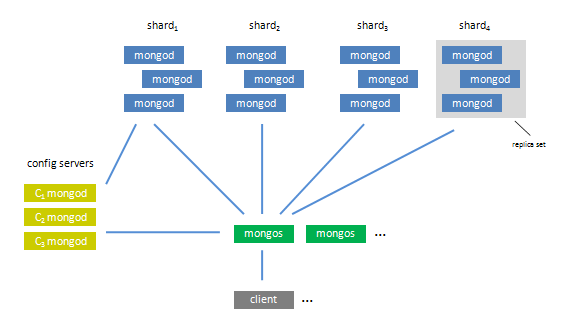
\includegraphics[width=1\textwidth]{chapters/technical-manual/sharding.png}
    \caption{MongoDB sharding}\label{sharding}
  \end{figure}
\end{description}

Vemos, pues, que MongoDB nos ofrece un buen balance de características
junto a una gran facilidad de uso. Podemos empezar a usar un único
servidor MongoDB y luego emplear \emph{replica sets} más
\emph{sharding}. Por eso, finalmente hemos elegido esta base de datos.

\subsection{DARE como procesos sin estado}

En el diseño de DARE hemos tratado de utilizar procesos sin estado y
una arquitectura en la que no se comparta el estado, \emph{shared
  nothing architecture}. Esto permite poder añadir procesos con
facilidad. También es una arquitectura más fiable, si un proceso falla
la siguiente petición puede ir a otro proceso del mismo tipo. La
escalabilidad de DARE por tanto se basa en un modelo basado en
procesos. Idealmente será responsabilidad del Sistema Operativo
relanzar los procesos que hayan terminado inesperadamente su
operación. La gran ventaja de este modelo es que para escalar
simplemente hay que lanzar más procesos ya sea en el mismo u otros
nodos.

Para ofrecer una mayor facilidad de administración los procesos Web
DARE son auto-contenidos. En vez de desplegar a un contenedor de
servlets existente, el artefacto
\emph{DARE-web<version>-standalone.jar} contiene todo lo necesario
para ejecutar un servidor web. Para ello se utiliza Jetty, que está
especialmente pensado para ser usado en modo embebido.

Hemos dicho que DARE utiliza procesos sin estado para llevar a cabo
sus actividades. Más concretamente habría dos tipos de procesos:
\begin{description}
  \item[Proceso Web:] Es fruto de ejecutar
    \emph{DARE-web<version>-standalone.jar}. Contiene Jetty, la
    aplicación web y la parte cliente de DARE-workers. Su número
    dependerá de las necesidades de escalabilidad.
  \item[Proceso Worker:] Es el fruto de ejecutar
    \emph{DARE-workers-<version>-standalone.jar}. Es responsable de
    realizar las ejecuciones de robots demandadas. Su número dependerá
    del número de ejecuciones necesarias a realizar.
\end{description}

\subsubsection{Arquitectura Backend}

En DARE llamamos \emph{Backend} a la parte responsable de almacenar
los datos y mandar las ejecuciones a aAUTOMATOR. La implementación de
esta parte se ha dividido en dos componentes: DARE-backend y
DARE-workers. Ver \ref{COMPONENTES-DARE},
pág.~\pageref{COMPONENTES-DARE}. Pero antes veamos la problemática a
afrontar y los principios por los que se guiará su implementación.

La base de datos elegida, MongoDB\ref{ELECCION-MONGO}, se encarga de
almacenar los datos. La única dificultad se presenta en convertir los
datos del dominio definidos en Java a documentos JSON y viceversa.
%TODO añadir referencia a DARE-domain

Por otro lado hay que distribuir la carga de las ejecuciones
solicitadas. Éste es un problema \emph{embarrassingly
  parallel}\cite{EMBARRASSINGLY-PARALLEL}. Cada ejecución es
completamente independiente de las otras, por lo que no hace falta
mantener una comunicación entre ellas. Esto nos permite tener un
modelo de escalabilidad muy sencillo. Simplemente hay que añadir más
threads o procesos. Finalmente nos hemos decantado por está última
opción ya que nos permite recargar la carga entre varios equipos.

El problema de utilizar procesos es que la comunicación es más
compleja. Una buena opción es utilizar el patrón
\emph{master-worker}\cite{MASTER-WORKER}. Básicamente hay procesos que
pondrían en una cola peticiones de trabajo a realizar y los
trabajadores tomarían esas peticiones de trabajo de la cola una vez
estuvieran listos. En el caso que nos ocupa hemos utilizado una ligera
variante de este patrón. En vez de introducir una nueva dependencia
usando una cola, el proceso \emph{master}\footnote{Proceso Web en este
  caso} proporciona directamente a uno de los workers la petición a
realizar. En cada momento se escoge el worker que tenga una menor
carga.

Aquí surge una nueva problemática: el proceso web necesita saber que
workers están disponibles. Se podrían utilizar muchas tecnologías,
pero como queríamos evitar introducir más dependencias optamos por
utilizar el sistema de almacenamiento. Así pues, cuando un worker
arranca registra su dirección IP y el puerto en el que está
escuchando. Los procesos web comprueban periódicamente que los
procesos worker gozan de buena salud y mandan las peticiones a los que
están menos ocupados.

Lo bueno de utilizar procesos sin estado es que podemos aumentar y
disminuir el número de procesos web y procesos worker según el tipo de
la carga de trabajo y la demanda del momento. La ventaja fundamental
de que sean procesos en vez de threads\footnote{hilos de ejecución} es
que podemos añadir también nuevos nodos físicos sin perturbar los que
ya están lanzados.

\subsection{Clojure como lenguaje de programación}

Clojure es un lenguaje de programación que se ejecuta sobre la
JVM\footnote{\emph{Java Virtual Machine}}, el
CLR\cite{CLR}\footnote{\emph{Common Language Runtime}} y
JavaScript. Para este proyecto nos interesa la implementación que se
ejecuta sobre la JVM y nos referiremos a ella de ahora en adelante.

Es un lenguaje de propósito general que combina la facilidad de uso de
un lenguaje de scripting con una infraestructura robusta y eficiente
para programación concurrente. Clojure es compilado a JVM bytecode
pero aun así es completamente dinámico: cualquier característica es
soportada en tiempo de ejecución.

Clojure es un dialecto de Lisp\cite{LISP} y comparte con Lisp la
filosofía de código como datos. Ofrece, pues, un poderoso sistema de
macros. Su paradigma es eminentemente funcional ofreciendo unas
estructuras de datos inmutables y
persistentes\cite{PERSISTENT-DATA-STRUCTURES}. Cuando mutabilidad es
necesaria, Clojure ofrece memoria transaccional y un sistema de
agentes reactivos\footnote{Es similar a un Actor en Erlang}.

Clojure ofrece facilidad de acceso a librerías Java, permitiendo
reutilizar una gran cantidad de código existente. Esto le confiere ser
práctico en gran medida.

Hemos empleado Clojure en DARE-backend y DARE-workers. La razón es que
intuíamos que Clojure nos ofrecería una productividad superior. Ha
sido una experiencia muy positiva. Creemos que el código resultante es
mucho más conciso y fácil de modificar que el equivalente en Java. El
mayor problema a destacar fue la poca familiaridad con Clojure en un
primer momento.

\subsubsection{Librerías Empleadas}
\begin{description}
\item[CongoMongo]\cite{CONGO-MONGO} es un envoltorio sobre el driver
  oficial Java de MongoDB. Nos ofrece una API más adecuada para ser
  usada desde Clojure.
\item[Lamina] es una librería para trabajar con eventos como si fueran
  secuencias. Se podría decir que sigue un paradigma funcional
  reactivo\cite{FRP}. Es la base sobre la que Aleph y Gloss se
  asientan. La abstracción clave es un \emph{channel}. Combina una
  cola con el patrón publicar/subscribir.
\item[Aleph] es una librería para realizar
  I/O\footnote{Entrada/Salida} asíncrona con varios protocolos: HTTP,
  WebSockets, TCP, UDP, etc. Representa la comunicación con un
  \emph{channel} de Lamina. Aleph permite realizar una comunicación
  asíncrona de manera sencilla.
\item[Gloss] es una DSL para definir formatos de
  comunicación. Convierte un flujo de bytes en estructuras de datos
  Clojure. Esto nos facilita parsear las peticiones realizadas en vez
  de tener que trabajar con el flujo de bytes proveniente de TCP. Por
  ejemplo, para dividir el flujo de bytes en peticiones de strings se
  puede hacer definiendo un \emph{codec} en Gloss. En la
  figura~\ref{gloss-example}, pág.~\pageref{gloss-example}, se define
  que cada petición sera una String codificada en UTF-8 con un entero
  indicando el tamaño de la misma.
  \begin{figure}[hb]
    \begin{center}
      \begin{minted}{clojure}
      (defcodec protocol-frame
        (finite-frame :int32 (string :utf-8)))
        \end{minted}
    \end{center}
  \caption{Ejemplo uso Gloss}\label{gloss-example}
  \end{figure}
\end{description}

\subsection{Librería para Python}

Hemos decidido hacer una librería para Python aparte de una en
Java. La idea es poder ofrecer una alternativa más sencilla que
Java. Python nos permite que el programador tenga un ejemplo
funcionando en menor tiempo. Además sus tiempos de arranque son
pequeños, lo que nos permite que sea la base para crear una aplicación
de línea de comandos.

Python es un lenguaje muy legible. Soporta varios paradigmas,
imperativo, OOP\footnote{\emph{Object Oriented Programming}}, y
funcional. Además cuenta con numerosas librerías de gran calidad lo
que siempre lo hace una opción interesante.

Una duda que nos asaltó fue si utilizar la versión 3 de Python. Es la
última versión del lenguaje y cuenta con ciertas mejoras pero su
presencia no es tan ubicua. Finalmente este último aspecto nos ha
decantado a favor de Python 2.

\subsubsection{httplib2}

Para realizar la librería hemos empleado httplib2. Esta librería
cliente HTTP nos ofrece ventajas con respecto a las librerías
incluidas por defecto en la distribución de Python. Las librerías
incluidas httplib y urllib son de nivel más bajo. Tendríamos, por
ejemplo, que manejar ciertos aspectos de HTTP como caching
manualmente.

Más concretamente httplib2 nos ofrece:
\begin{description}
  \item[Soporte Keep-Alive]: Permite mantener el mismo socket abierto
    y reutilizarlo para hacer varias peticiones.
  \item[Soporte Autenticación]: Soporta varios tipos de
    autenticación HTTP como Digest, Basic y WSSE.
  \item[Soporte cacheado]: Tiene una caché privada que se conserva
    entre requests. Entiende la cabecera Cache-Control y los
    validadores ETag y Last-Modified.
  \item[Soporte métodos HTTP]: Soporta todos los métodos HTTP, no solo
    GET y POST.
  \item[Soporte Redirects]: Procesa automáticamente los redirects
    devueltos por el servidor web.
  \item[Soporte Comprensión]: Puede recibir respuestas comprimidas ya
    sea con comprensión deflate o gzip.
\end{description}

\subsection{Interfaz Línea Comandos en Python}

La idea es poder ofrecer una aplicación que permita emplear DARE de
una manera sencilla y directa. Además nos permitía probar la librería
en un caso de uso real. Hemos empleado la librería en Python DARE para
realizarla. Python dispone además de librerías muy completas para el
manejo y parseado de argumentos como argparse. Por brevedad, nos
referiremos de ahora en adelante a esta aplicación \emph{dare.py}.

Una característica que queríamos añadir a esta aplicación es la
posibilidad de recordar los robots y los resultados que has tenido
anteriormente. Creemos que esto facilitaría en gran medida el trabajo
al usuario, podría ver los robos que ha creado y los resultados
obtenidos. Para ello necesitamos un sistema de almacenamiento que
conserve esos datos entre diferentes invocaciones a \emph{dare.py}.

\subsubsection{SQLite}

Para realizar esta labor de almacenamiento nos hemos decantado por
SQLite\cite{SQLite}. SQLite nos ofrece una base de datos relacional en
la forma de una librería de tamaño reducido, permitiéndonos usarla en
modo embebido. Es muy fácil de usar, no requiere configuración para
empezar a ser usada y su rendimiento es de sobra adecuado para nuestra
necesidad concreta.

Es muy usada como sistema de almacenamiento local, justo el caso que
nos ocupa.

\subsection{Componentes}
\label{COMPONENTES-DARE}
A continuación veamos una visión general del proyecto desde el punto
de vista de un diagrama de componentes UML. En el se muestran los
componentes presentes y las relaciones entre los mismos. A mayores
vamos a realizar una breve descripción de cada uno de ellos:

\begin{description}

\item[minilenguaje:] Es el componente que implementa la DSL definida
  por el proyecto. Este lenguaje se ha denominado minilenguaje. Es
  responsable de transformar la DSL en el formato XML entendido por
  \emph{aAUTOMATOR Runtime}\footnote{Está contenido dentro del
    artefacto \emph{StringEditor}}. Está implementado en JRuby y
  Java. La parte en JRuby se encarga de definir una DSL interna y la
  parte Java ofrece una API a la misma.
\item[DARE-domain:] Define un modelo de dominio del sistema. Facilita
  una comprensión conceptual del sistema, abstrayéndonos de otras
  consideraciones. Contiene clases como Robot, ExecutionResult y
  PeriodicalExecution. Instancias de estas clases son creadas cuando
  se obtienen datos del sistema de almacenamiento. Está implementado
  en Java.
\item[DARE-war:] Es una aplicación web Java. Contiene todos los
  componentes dentro del recuadro servicio. Puede ser desplegado en
  cualquier servidor de aplicaciones JEE y/o contenedor de servlets.

  Siguiendo el patrón MVC\footnote{Modelo Vista Controlador} este
  modelo es el responsable de la parte de vista y controlador. Utiliza
  la API JAX-RS para lleva a cabo esta labor. Utiliza a DARE-domain
  como modelo y DARE-backend ofrecería servicios de persistencia y
  ejecución.

  Este componente ha sido concebido de modo que se puede desplegar en
  varios nodos, ya que se sigue una filosofía
  \emph{share-nothing}. Para ellos nos hacemos valer de las
  características sin estado de REST. Es decir, podemos tener varios
  servidores web ejecutándose en distintos nodos. Está implementado en
  Java.

\item[DARE-backend:] Es el componente encargado de comunicarse con la
  base de datos MongoDB tanto para leer como para escribir los objetos
  definidos en DARE-domain. Recibe también las peticiones de ejecución
  para aAUTOMATOR. Luego utilizando la parte cliente de DARE-workers
  las reparte entre los procesos \emph{worker} que se están
  ejecutando. Está implementado en Clojure.

\item[DARE-workers:] Este componente está compuesto por una parte
  cliente que lanza peticiones de ejecución a aAUTOMATOR. La parte
  servidor, de ahora en adelante \emph{worker}, interpreta esas
  peticiones y hace el trabajo correspondiente. Uno o varios de estos
  workers pueden estar lanzados en función de las necesidades de
  escalabilidad y fiabilidad necesarios.

  Cada worker es un proceso, por lo que alguno de ellos podría dejar
  de funcionar y DARE podría seguir ofreciendo su servicio. Además al
  ser cada uno un proceso se pueden ejecutar localmente en el mismo
  nodo o repartirlo a través de varios nodos del cluster. La parte
  cliente es capaz de descubrirlos y repartir la carga de peticiones
  entre los workers. Aparte comprueba continuamente el estado de salud
  de los workers para que el servicio continúe funcionando aun en la
  presencia de errores en los workers.

 Tanto la parte servidor como cliente están implementados en Clojure.

\item[DARE-util:] Es un cajón de sastre donde se encuentran diversas
  funciones de utilidad usadas por otros módulos.

\item[DARE-web:] Este módulo se utiliza para facilitar el despliegue
  de la aplicación. Toma el fichero \emph{war} con la aplicación y lo
  ejecuta creando un servicio web. Para ello emplea el contenedor de
  servlets embebido, Jetty\cite{JETTY}. Jetty es un contenedor de
  servlets ligero, por lo que es especialmente adecuado para lanzar
  numerosas instancias de la aplicación. Este componente está
  implementado en Clojure.

\item[DARE-java:] Este módulo implementa la librería cliente para
  Java. Utiliza JAX-RS para implementar su funcionalidad. Para
  facilitar su implementación se han incluido algunas clases de
  DARE-war, más concretamente las clases de la parte de vista. Al
  compartir estas clases con DARE-web se facilita el mapeado de las
  respuestas por parte de JAX-RS.

  Aparte está librería se utiliza para realizar los tests funcionales
  de DARE-war.
\item[DARE-python:] Este módulo implemente la librería cliente para
  Python, así como la aplicación de línea de comandos. Como se ha
  descrito anteriormente usa httplib2 para llevar a cabo la
  comunicación con el servicio.

  La aplicación de línea de comandos está contenida en este componente
  y utiliza la librería creada para llevar a cabo su
  funcionalidad. Como es lógico está implementado en Python.
\end{description}

\begin{landscape}
\begin{figure}[p]
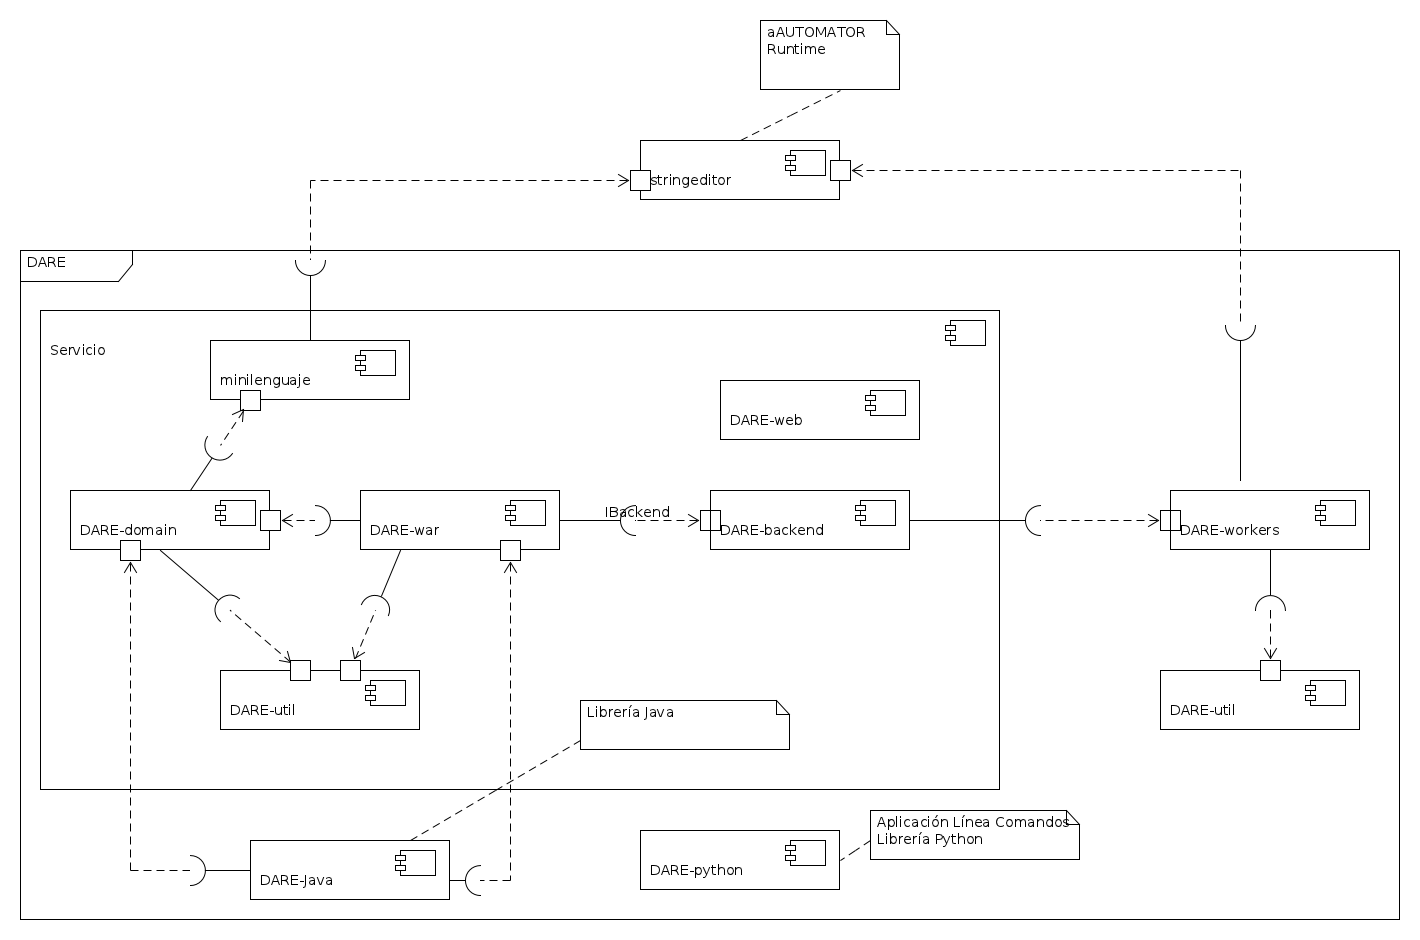
\includegraphics[width=1.4\textwidth]{chapters/technical-manual/diagrams/diagrama_componentes.png}
\caption{Diagrama Componentes DARE}\label{diagrama_componentes_dare}
\end{figure}
\end{landscape}

\subsubsection{Diagrama clases minilenguaje}

En este diagrama mostramos las clases con las que se implementa la DSL
interna propuesta.

Por un lado tenemos la clase \emph{Transformer}. Un objeto de esta
clase se corresponde a uno de los transformadores de los que está
compuesto un robot. Ver~\ref{COMPORTAMIENTO_AUTOMATOR},
pág.~\pageref{COMPORTAMIENTO_AUTOMATOR}. Sigue el patrón
Composite\cite{COMPOSITE_PATTERN}, es decir, cada \emph{Transformer}
puede a su vez tener \emph{Transformers} hijos. Cada
\emph{Transformer} es capaz de convertirse al XML que necesita
aAUTOMATOR. Cada subclase de \emph{Transformer} se corresponde a una
clase \emph{Transformer} de aAUTOMATOR. Cada \emph{Transformer} va a
necesitar una serie de parámetros requeridos y opcionales. Cada
subclase de \emph{Transformer} define pues, los parámetros que va a
necesitar de una manera declarativa. \emph{Transformer} mantiene una
lista de los hijos que contiene y permite que se le añadan más. Además
puede recibir un XML de aAUTOMATOR y convertirlo a una \emph{string}
de minilenguaje que produciría ese XML.

La clase \emph{Language} es la encargada de procesar el
lenguaje. Básicamente el lenguaje se evalúa contra una instancia de
\emph{Language}. Por ejemplo, el minilenguaje definido por
\emph{xpath('//a/@href')} implica que el método xpath de
\emph{Language} es llamado. ¿Implica esto que habría que definir
métodos por cada \emph{Transformer} que se defina? No, empleando
meta-programación\cite{METAPROGRAMMING} cada vez que se define una
subclase de \emph{Transformer} se crea dinámicamente un nuevo método
en \emph{Language}. Llamar a este método implica crear el
\emph{Transformer} de la subclase adecuada con los parámetros
indicados. En este momento el \emph{Transformer} creado se añade al
que está ligado al de \emph{Language}. Es decir, según se van llamando
a los métodos que crean los transformers estos se van añadiendo al
transformer de primer nivel en el \emph{Language}. Por ejemplo,
\emph{url | xpath('//a/@href') | patternMatcher('(http://.*)')} añade
tres \emph{Transformers} al \emph{Transformer} padre, que por defecto
está en modo cascade. Como se puede ver se emplea el operador \emph{|}
para separar cada \emph{Transformer}. Esto no es más que azúcar
sintáctico. El siguiente ejemplo sería equivalente: \emph{url;
  xpath('//a/@href'); patternMatcher('(http://.*)')}, pero con el
operador \emph{|} queda más clara la intención.

\emph{Language} tiene los métodos \emph{pipe} y \emph{branch}. Estos
métodos definen un nuevo \emph{Transformer} con semánticas de CASCADE
o de BRANCH. Por tanto, para \emph{branch} se requiere indicar el
BRANCH~TYPE y el MERGE~MODE. Estas llamadas crear un nuevo
\emph{Language} con su correspondiente \emph{Transformer}. Estos
métodos reciben un bloque de código que se interpretará en el contexto
de la nueva instancia de \emph{Language}.

\emph{DocumentWrapper} y \emph{AttributesWrapper} se encargan de
facilitar la generación del XML.

Todas estas clases están definidas en el fichero
\emph{minilanguage/src/main/resources/es/uvigo/ei/sing/stringeditor/transformer.rb}.

\begin{landscape}
\begin{figure}[hp]
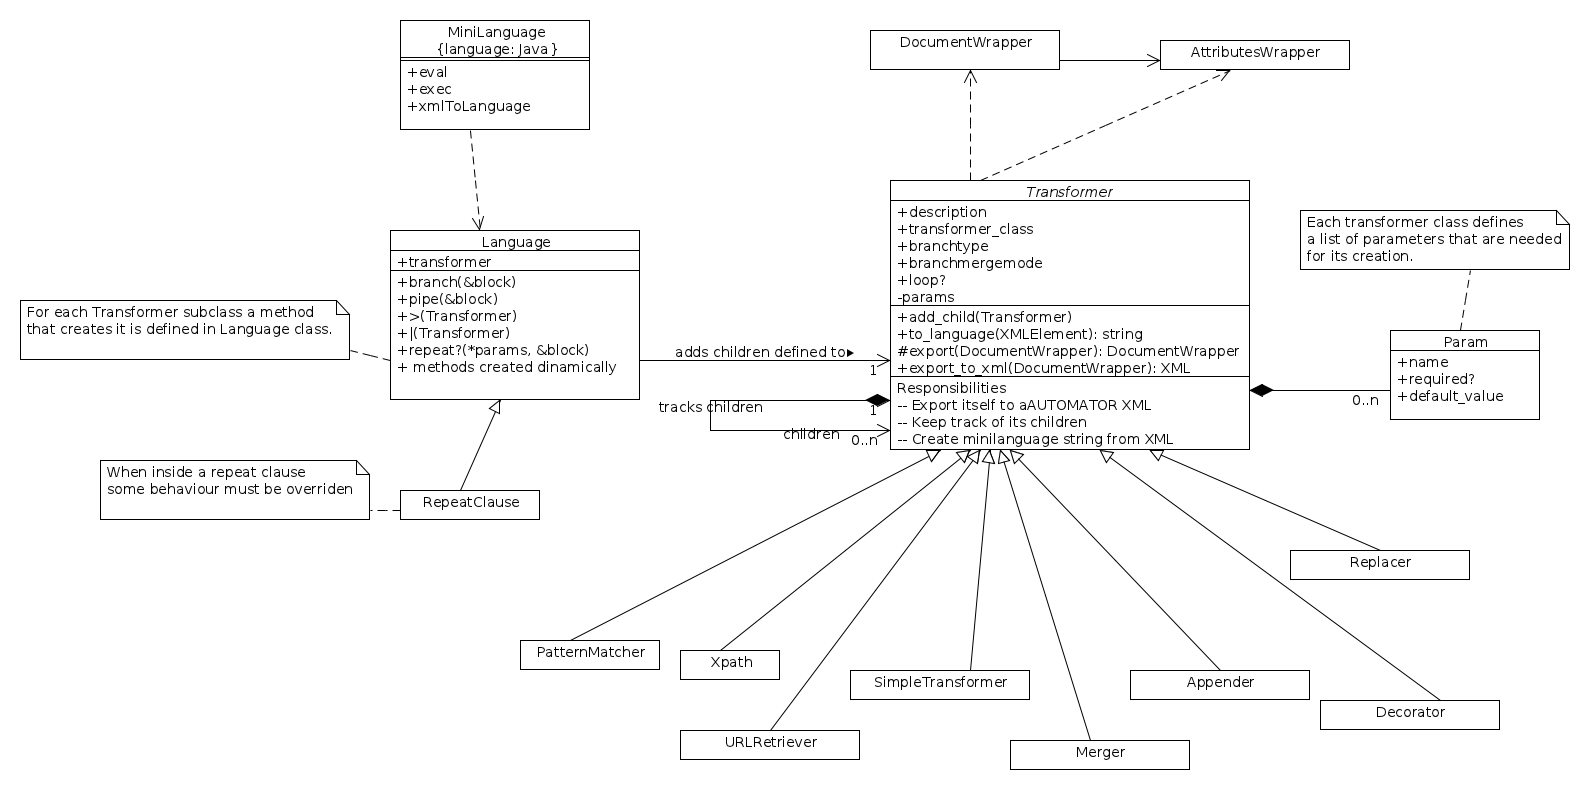
\includegraphics[width=1.4\textwidth]{chapters/technical-manual/diagrams/clases_minilenguaje.png}
\caption{Diagrama clases Minilenguaje}\label{diagrama_clases_minilenguaje}
\end{figure}
\end{landscape}

\subsubsection{Descripción Implementación Minilenguaje}

Después de la introducción a minilenguaje apoyada en el diagrama de
clases hemos creído conveniente utilizar algunas técnicas adicionales
para facilitar su comprensión. La implementación de una DSL interna es
difícil de capturar con un diagrama de clases, por lo que hemos
buscado otras formas de exponer su comportamiento.

Más concretamente hemos optado por aplicar Docco\cite{DOCCO} a la
implementación. Docco nos permite aplicar técnicas de programación
literaria\cite{LITERATE_PROGRAMMING}.

Al realizar programación literaria se escribe un ensayo en lenguaje
natural con segmentos de código intercalados. La herramienta de
programación literaria genera a partir de este documento código apto
para ser ejecutado o compilado. El programador al no tener que
producir directamente el producto final a ser compilado, puede exponer
el razonamiento y las abstracciones detrás de un programa de la manera
más adecuada para los posibles lectores. En vez de seguir una
estructura impuesta por el compilador se persigue la estructura más
adecuada para transmitir las ideas subyacentes.  De este modo se
facilita la comprensión del programa.

Docco persigue objetivos similares pero sin realizar un proceso de
transformación del código fuente. Esto facilita la introducción de
técnicas de programación literaria utilizando herramientas típicas. Si
bien no es estrictamente programación literaria, se alcanzan muchos de
sus objetivos. Por ejemplo, muchas veces para lograr una exposición
adecuada del programa se requiere la modificación de su estructura
para que sea acorde con el ensayo generado.

Docco por defecto genera este ensayo en forma de HTML, para la
inclusión del mismo en este proyecto hemos modificado Docco para
producir \LaTeX{}\cite{DOCCOTEX}.

Por último señalar que la documentación producida está en inglés ya
que el código esta en ese mismo idioma.

\begin{landscape}
\begingroup
    \fontsize{9pt}{11pt}\selectfont
    \input{doccotex/transformer.tex}
\endgroup
\end{landscape}

\subsubsection{Diagrama clases DARE-domain}

En el diagrama de clases de entidades,
\ref{diagrama_clases_entidades_domain}
pág.~\pageref{diagrama_clases_entidades_domain}, se muestran las
entidades por las que está formada la aplicación. Por cada
\emph{Robot} puede haber cero, uno o varios
\emph{ExecutionResult}. Por cada \emph{ExecutionResult} hay un
\emph{Robot}. Por cada \emph{Robot} puede haber cero, uno o varios
\emph{PeriodicalExecution}. Por cada \emph{PeriodicalExecution} hay un
\emph{Robot}. Una \emph{PeriodicalExecution} no contiene un
\emph{ExecutionResult} si todavía no se ha completado la
ejecución. Una vez se ha completado el \emph{PeriodicalExecution}
contiene el \emph{ExecutionResult} de su última ejecución.

\emph{Robot} llama a MiniLanguage para generar el XML de aAUTOMATOR a
partir del minilenguaje que haya sido creado. Contiene métodos para
crear tanto un nuevo \emph{ExecutionResult} como una nueva
\emph{PeriodicalExecution}. Un \emph{Robot} no contiene directamente
las \emph{PeriodicalExecution} y los \emph{ExecutionResult}
asociados. Las asociaciones solo indican la cardinalidad existente. El
\emph{ExecutionResult} no contiene una referencia al \emph{Robot}
asociado, solo guardan el código del \emph{Robot}
asociado. \emph{PeriodicalExecution} si que contiene su
\emph{ExecutionResult} asociada.

Por lo demás DARE-Domain define una serie de interfaces y clases de
utilidad usadas por DARE-war. La interfaz clave es \emph{IBackend}. La
implementación de esta interfaz debe ser capaz de eliminar y guardar
las entidades definidas por DARE-Domain. Se definen dos excepciones
que se pueden producir relacionadas con el manejo de
ejecuciones. \emph{IBackendBuilder} define una interfaz para el objeto
que debe de crear el \emph{IBackend} a ser usado. Define y acepta una
serie de parámetros necesarios para la operativa concreta del backend
seleccionado.

La clase \emph{Maybe} sirve para indicar que un resultado es
opcional. Por otra parte \emph{MinilanguageProducer} sirve para mantener una
lista de instancias de \emph{Minilanguage} preparadas para ser
usadas. Ver~\ref{interpreter_state_manipulation},
pág.~\pageref{interpreter_state_manipulation}.

\begin{landscape}

\begin{figure}[hp]
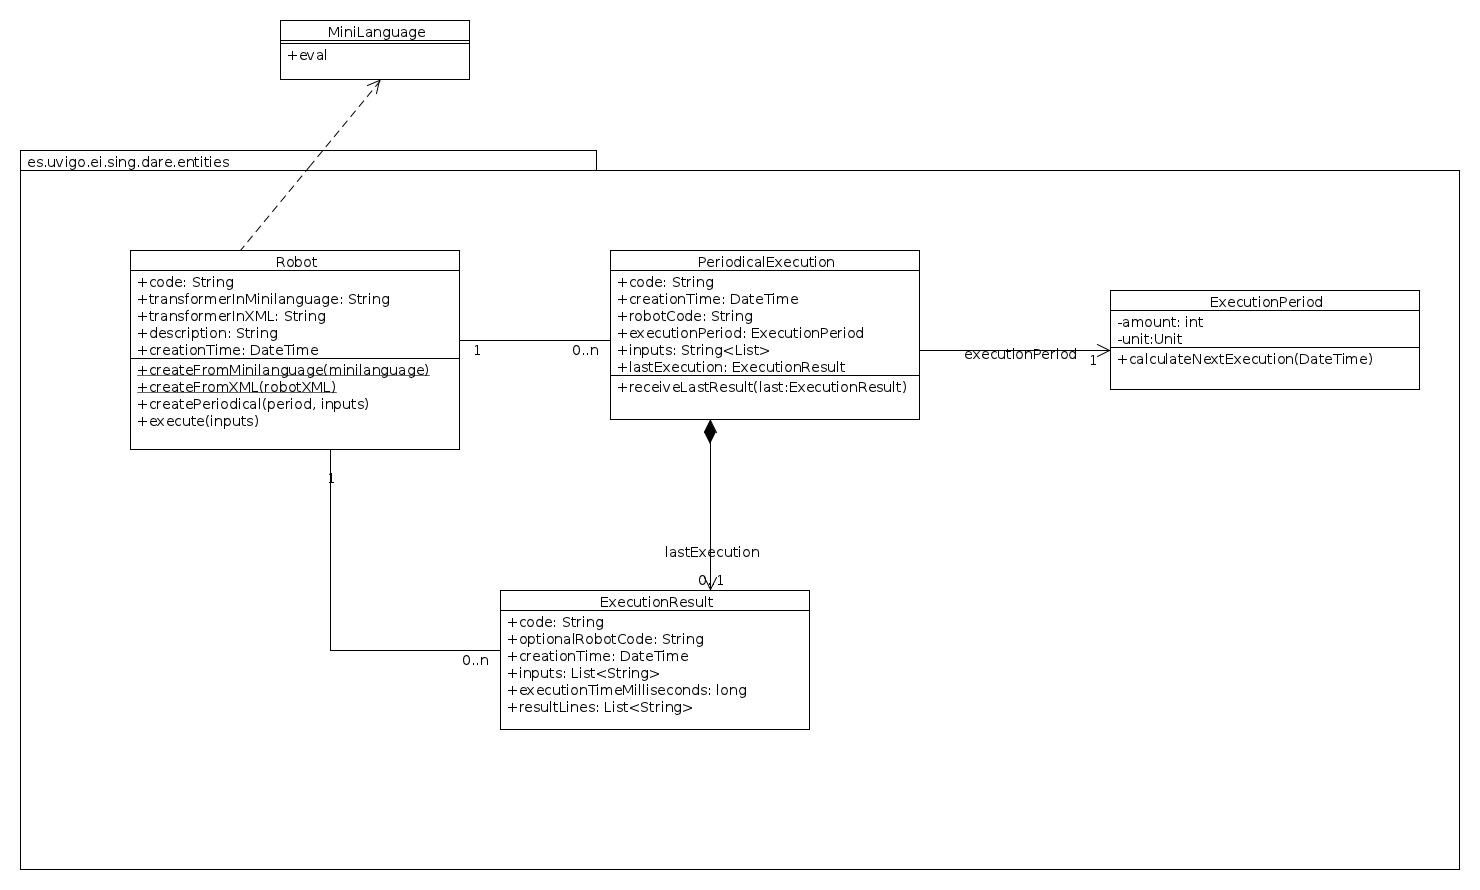
\includegraphics[width=1.4\textwidth]{chapters/technical-manual/diagrams/entidades_domain.png}
\caption{Diagrama clases detallado de Entidades}\label{diagrama_clases_entidades_domain}
\end{figure}

\begin{figure}[hp]
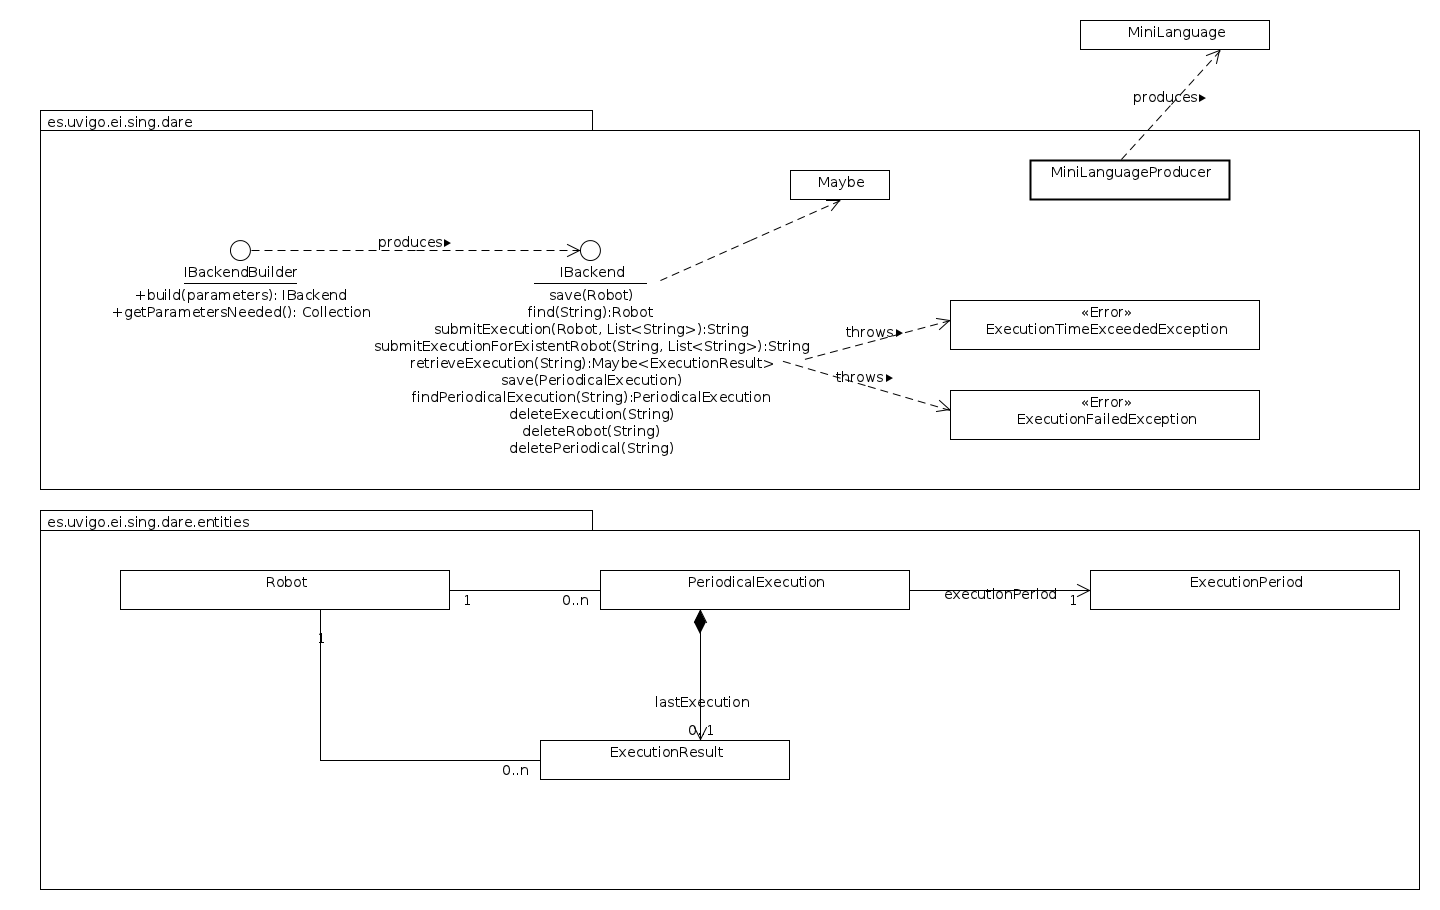
\includegraphics[width=1.4\textwidth]{chapters/technical-manual/diagrams/clases_domain.png}
\caption{Diagrama clases Domain}\label{diagrama_clases_domain}
\end{figure}

\end{landscape}

\subsubsection{Diagrama clases DARE-war}

Se muestran las clases de este componente agrupadas en paquetes junto
a clases de otros componentes que son de interés.

\emph{ConfigurationBootstrapper} es una clase que a partir del
contexto web crea un objeto \emph{Configuration}. Este objeto se
guarda en el contexto de la aplicación web y está disponible para los
recursos. El objeto \emph{Configuration} tiene referencias a la
implementación de \emph{IBackend} que se va a usar y el
\emph{MinilanguageProducer}.

En el paquete resources están definidas varias clases que definirán
los recursos REST de los que se compone la aplicación web. Vienen a
cumplir la función de controladores y utilizan la librería
JAX-RS. Estos controladores utilizan \emph{IBackend} para guardar y
obtener las entidades. Además le piden a \emph{IBackend} que se
realicen ejecuciones. Como resultados de algunas operaciones de
lectura se crean objetos del paquete views.

En el paquete views están definidos varios objetos con escasa lógica
que definen estructuras de datos que se van a traducir a XML y
JSON. La estructura de estas clases y del JSON o XML generado es la
misma. Para hacer la traducción JAX-RS utiliza JAXB\cite{JAXB}.

\begin{landscape}
\begin{figure}[hp]
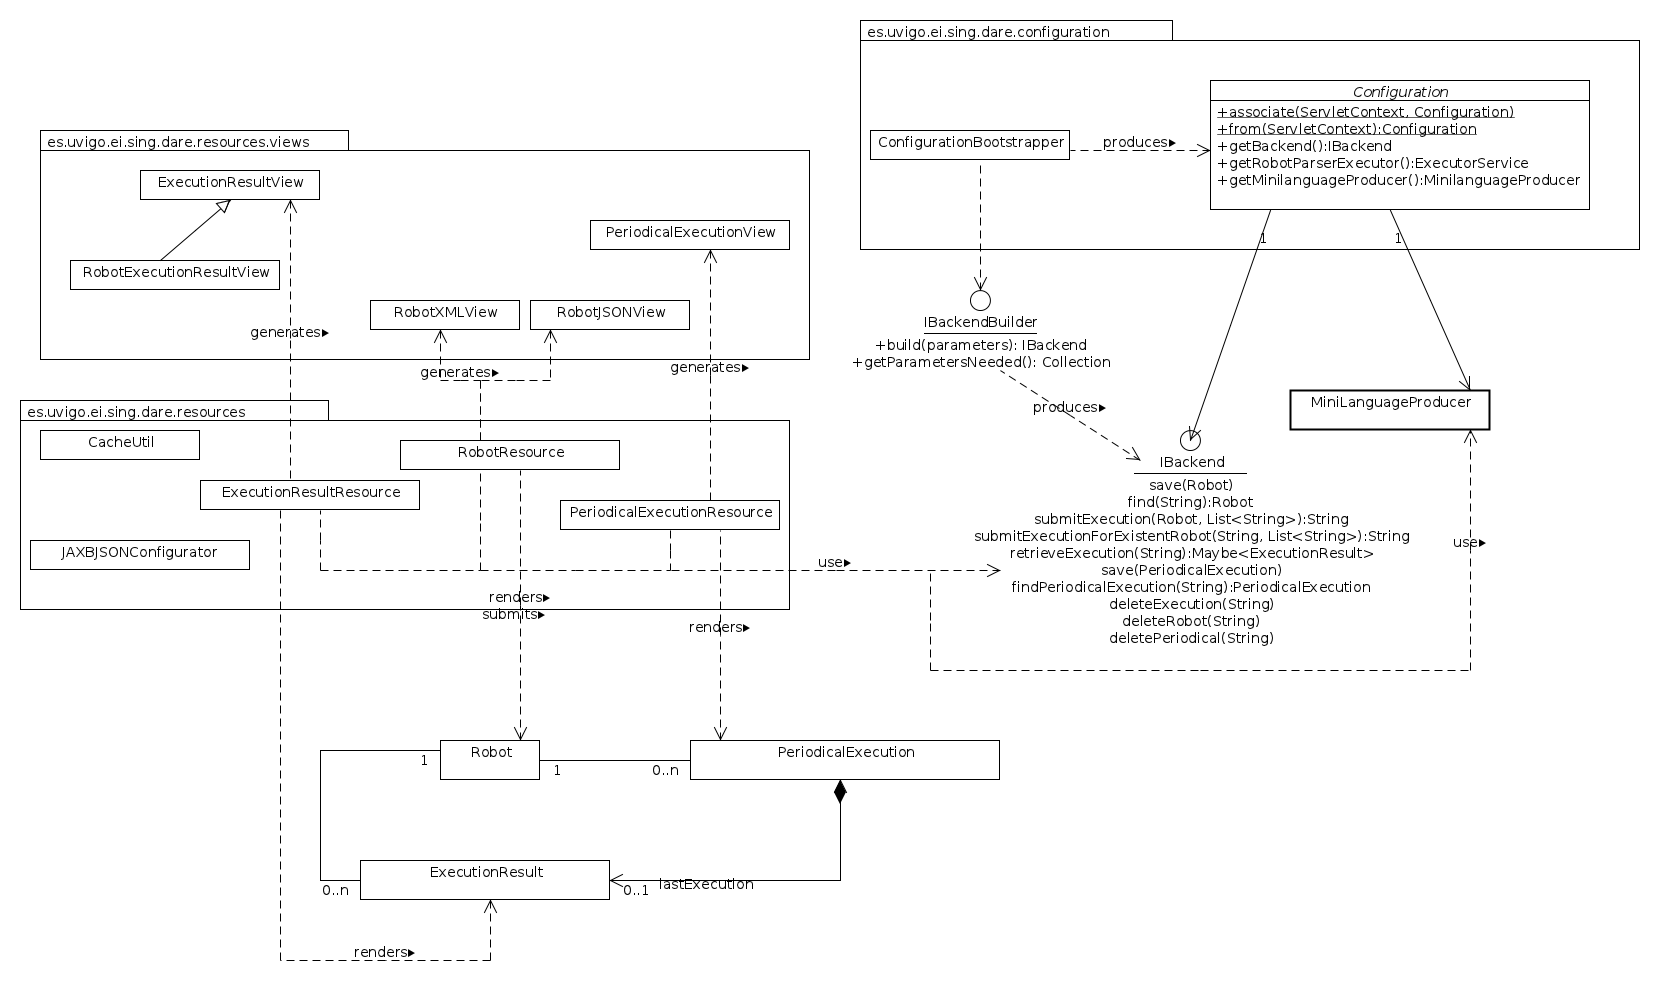
\includegraphics[width=1.4\textwidth]{chapters/technical-manual/diagrams/clases_war.png}
\caption{Diagrama clases WAR}\label{diagrama_clases_war}
\end{figure}
\end{landscape}

\subsubsection{Diagrama clases DARE-backend}
% a fondo backend/core.clj?
\subsubsection{Diagrama clases DARE-workers}
% a fondo workers/client.clj, workers/server.clj?

\subsubsection{Diagrama clases DARE-java}
A continuación~\ref{diagrama_clases_dare_java} mostramos un diagrama
de clases de la librería para acceder a DARE desde Java. La clase DARE
contiene métodos para crear nuevas entidades y para acceder a las
mismas. Internamente se usa JAX-RS, más concretamente a través de una
instancia de Client. Se reutiliza el paquete de vistas de DARE-war. La
clase DARE puede devolver instancias de las mismas para ser consumidas
por los clientes de la librería. Como se puede observar en el diagrama
la clase DARE utiliza la clase URIPoller. Esta clase facilita se
encarga de hacer el \emph{polling} necesario para obtener ejecuciones
todavía en curso.

\begin{figure}[hp]
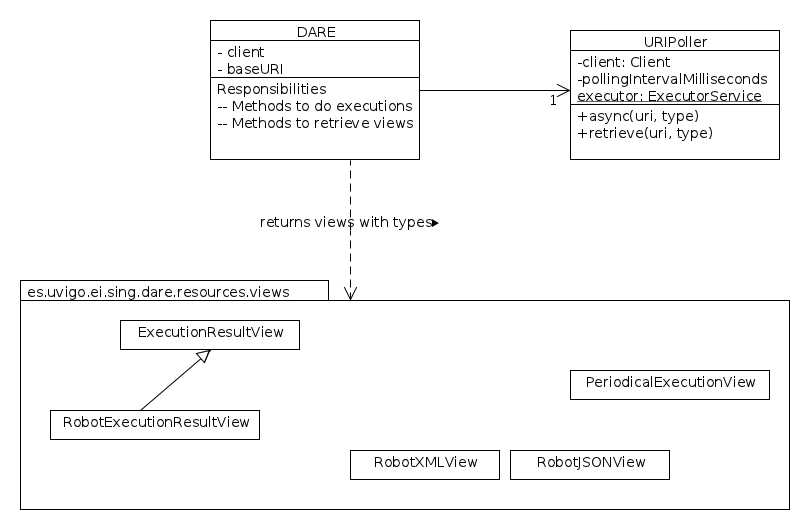
\includegraphics[width=\textwidth]{chapters/technical-manual/diagrams/clases_dare_java.png}
\caption{Diagrama clases DARE-java}\label{diagrama_clases_dare_java}
\end{figure}

\subsubsection{Diagrama clases DARE-python}

La clase Server contiene varios métodos para realizar acciones en el
servidor. Sobre esta clase de modelan varias clases que serán los
recursos de los que consta DARE. Cada uno de estos recursos tendrá
métodos para mostrar y eliminar un recurso. Cuando se muestra un
recurso a través del método \emph{show} se devuelve el objeto en
formato JSON. Aparte contienen métodos para generar otros recursos a
partir de ellos. Por ejemplo, a partir de un recurso \emph{Robot} se
puede generar una \emph{Execution} o una \emph{Periodical}. La clase
\emph{DARE} funciona a modo de punto de entrada del sistema. A partir
de este recurso se pueden crear recursos \emph{Robot} o
\emph{Execution}.

La funcionalidad expuesta por esta jerarquía de clases se puede
utilizar desde la línea de comandos. La línea de comandos utiliza un
objeto \emph{Store} para almacenar las ejecuciones realizadas y los
robots creados. En el diagrama hemos mostramos una clase \emph{Main}
que se comunica con la jerarquía de recursos y la clase
\emph{Store}. En realidad esta clase no existe en el código, son una
serie de métodos definidos en \emph{DARE-python/rest.py} con las
responsabilidades indicadas en el diagrama.

\begin{landscape}
\begin{figure}[hp]
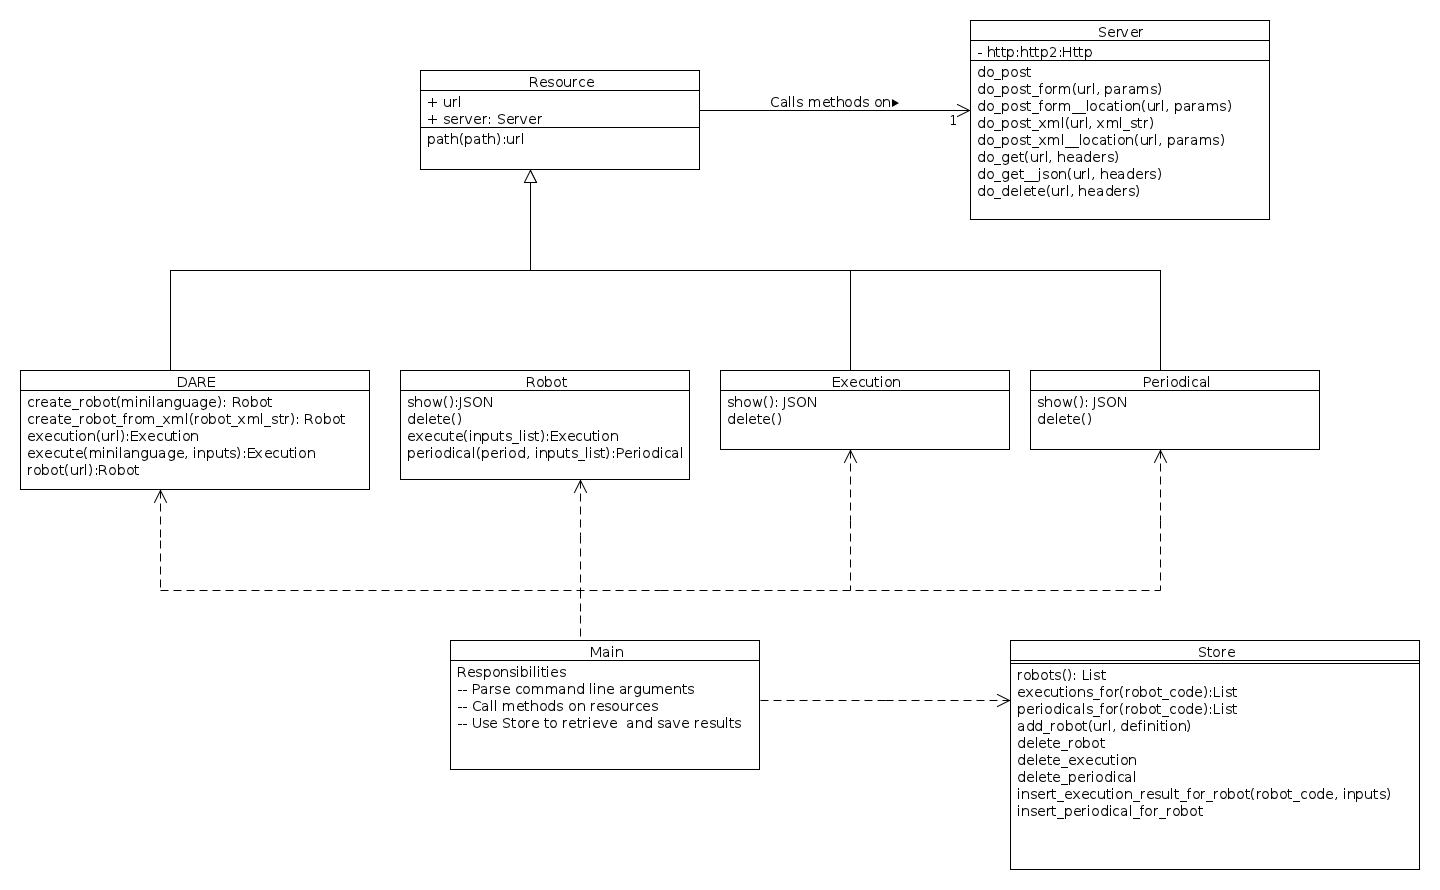
\includegraphics[width=1.4\textwidth]{chapters/technical-manual/diagrams/clases_dare_python.png}
\caption{Diagrama clases DARE-python}\label{diagrama_clases_dare_python}
\end{figure}
\end{landscape}

\subsubsection{Esquema datos Sistema Almacenamiento}

Vamos a describir los datos almacenados en MongoDB. Aunque MongoDB no
utiliza un esquema fijo de manera explícita si que se podría decir que
existe un esquema implícito. Este esquema describe los atributos que
la aplicación espera que estén presente en un documento del tipo
indicado. Para cada colección\footnote{Equivalente a tabla en una base
de datos relacional} describimos los campos que son requeridos por
DARE, el tipo de datos esperado y su semántica.

La clase de DARE-Domain \emph{Robot} es mapeada a la colección
\emph{robots}~\ref{robot_collection},
página~\pageref{robot_collection}.

La clase de DARE-Domain \emph{ExecutionResult} es mapeada a la
colección \emph{executions}~\ref{execution_collection},
página~\pageref{execution_collection}.

La clase de DARE-Domain \emph{PeriodicalExecution} es mapeada a la
colección \emph{executions}~\ref{periodical_execution_collection},
página~\pageref{periodical_execution_collection}.

\begin{table}[hbp]
\begin{tabularx}{\textwidth}{|l|l|l|X|}
\hline
Atributo & Tipo & Requerido & Descripción \\ \hline
\_id & string & Sí & La clave del documento. Se genera internamente en la
aplicación. Tiene formato de UUID. \\ \hline
creationTime & NumberLong & Sí. & Indica la fecha de creación a modo de
número de milisegundos desde \emph{epoch}. \\ \hline
description & string & No. & Texto acerca del cometido del
robot. \\ \hline
transformerInMinilanguage & string & Sí. & La versión en minilenguaje
del transformador. \\ \hline
transformerInXML & string & Sí. & La versión en XML del transformador. \\ \hline
\end{tabularx}
\caption{Colección Robot}
\label{robot_collection}
\end{table}

\begin{table}[hbp]
\begin{tabularx}{\textwidth}{|l|l|l|X|}
\hline
Atributo & Tipo & Requerido & Descripción \\ \hline
\_id & string & Sí & La clave del documento. Se genera internamente en la
aplicación. Tiene formato de UUID. \\ \hline
creationTime & NumberLong & Sí. & Indica la fecha de creación a modo de
número de milisegundos desde \emph{epoch}. \\ \hline
optionalRobotCode & string & Sí. & El código del robot al que
pertenece. El nombre es desafortunado debido a que el atributo se
llama igual que en la clase Java.\\ \hline
inputs & Array de string & Sí. & El vector de entrada
utilizado. \\ \hline
\multicolumn{4}{c}{Presentes después ejecución} \\ \hline
resultLines & Array de string & No. & El resultado
producido. \\ \hline
executionTimeMilliseconds & NumberLong & No. & El número de
milisegundos que llevo realizar la ejecución incluido tiempo de espera
en el \emph{worker}. \\ \hline
realExecutionTime & NumberLong & No. & El número de
milisegundos que llevo realizar la ejecución sin tiempo de espera
en el \emph{worker}. \\ \hline
\end{tabularx}
\caption{Colección Ejecución}
\label{execution_collection}
\end{table}

\begin{table}[hbp]
\begin{tabularx}{\textwidth}{|l|l|l|X|}
\hline
Atributo & Tipo & Requerido & Descripción \\ \hline
\_id & string & Sí & La clave del documento. Se genera internamente en la
aplicación. Tiene formato de UUID. \\ \hline
robotCode & string & Sí. & El código del robot al que
pertenece en formato UUID. \\ \hline
creationTime & NumberLong & Sí. & Indica la fecha de creación a modo de
número de milisegundos desde \emph{epoch}. \\ \hline
inputs & Array de string & Sí. & El vector de entrada a
utilizar. \\ \hline
executionPeriod & Object & Sí. & Un objeto con los campos amount y
unitType. Indica el periodo de ejecución.\\ \hline
lastExecution & Object & No & Un objeto con los mismos campos que una
\emph{Ejecución} menos optionalRobotCode. Ver
\ref{execution_collection}. \\ \hline
\multicolumn{4}{c}{Campos planificación} \\ \hline
next-execution-ms & NumberLong & Sí & Indica la fecha en la que se
debe de ejecutar esta ejecución periódica. Esta fecha se indica en
forma de número de milisegundos desde \emph{epoch}\\ \hline
scheduled & boolean & Sí & Si esta ejecución periódica ha sido marcada
para ser planificada y está a la espera de ser lanzada.\\ \hline
\end{tabularx}
\caption{Colección Ejecución Periódica}
\label{periodical_execution_collection}
\end{table}


\section{Pruebas}

A lo largo del desarrollo se han realizado diversos tipos de pruebas
automatizadas. Valoramos capturar los casos de prueba como código
ejecutable porque porque permiten detectar errores cuanto antes y no
requiere intervención manual.

\subsection{Pruebas unitarias}

Las pruebas unitarias comprueban que unidades aisladas de la
aplicación funcionan según lo especificado. Esta clase de tests son
útiles para detectar inmediatamente desviaciones con respecto al
comportamiento especificado. La mayoría de las pruebas de este tipo
que se han realizado son de caja blanca ya que se han diseñado
conociendo la estructura interna de la aplicación.

\subsubsection{Pruebas Minilanguage}

Se ha empleado RSpec\cite{RSPEC}. Es una herramienta para hacer tests
siguiendo el estilo BDD\footnote{\emph{Behaviour-Driven
    Development}}. Este estilo de TDD\footnote{\emph{Test-Driven
    Development}} hace un especial énfasis en generar especificaciones
legibles del software desarrollado. En el resultado de ejecutar
minilanguage/src/main/resources/es/uvigo/ei/sing/stringeditor/transformer\_spec.rb
se puede ver una lista de ejemplos que caracterizan el comportamiento
de
minilanguage/src/main/resources/es/uvigo/ei/sing/stringeditor/transformer.rb. Ver
el cuadro~\ref{rspec_tests}, página~\pageref{rspec_tests}.

\begin{table}[hbp]
\begingroup
    \fontsize{9pt}{11pt}\selectfont
\begin{verbatim}
aAUTOMATOR minilanguage
  Transformer
    should accept description
    description shouldn't be allowed to be changed once set
    should have transformer_class name as default value for description
    should accept branchtype parameter
    should have branchtype CASCADE as default
    should accept parameter branchmergemode
    should have branchmergemode SCATTERED as default
    should accept parameter loop
    should keep parameters
    should let add children
    must have an empty list as children initially
    should not let modify original children collection
    can have other transformers as children
      should report the added children
      it should behave like invariants for a Transformer
        should have a not nil description
        should have a not nil transformer_class
        should have a not nil branchtype
        should have a not nil branchmergemode
        should traverse tranformer
    PatternMatcher
      should have a fixed transformer class
      should require parameter pattern
      should read parameter pattern
      should let specify pattern as just one param
      should let specify additional params
      it should behave like invariants for a Transformer
        should have a not nil description
        should have a not nil transformer_class
        should have a not nil branchtype
        should have a not nil branchmergemode
        should traverse tranformer
  Language
    should let put transformers in cascade
    should let the language be supplied as a string
    should let put transformers as children of other transformer in cascade
    should let put several consecutive pipes
    should let put transformers in branch
    should let put transformers in branch as children of other transformer
    should not let use | inside a branch
    should let put transformers in cascade inside branch
    should let do a loop
    should let put several transformer serially connected in the repeat clause
    should let put several transformers paralelly connected in the repeat clause

Finished in 0.589 seconds
39 examples, 0 failures
\end{verbatim}
\endgroup
\caption{RSpec Tests para minilenguaje}
\label{rspec_tests}
\end{table}

\subsubsection{Pruebas DARE-domain}
Se ha empleado JUnit\cite{JUNIT} para realizar las pruebas de
DARE-domain. JUnit es un framework para realizar pruebas unitarias
para la plataforma Java. El resultado se puede ver en el
cuadro~\ref{junit_dare-domain},pág.~\pageref{junit_dare-domain}.

\begin{table}[hbp]
\begingroup
    \fontsize{9pt}{11pt}\selectfont
\begin{verbatim}
Testsuite: es.uvigo.ei.sing.dare.entities.ExecutionPeriodTest
Tests run: 9, Failures: 0, Errors: 0, Time elapsed: 0.124 sec

Testcase: anExecutionPeriodIsComposedOfAnAmountAndAnUnit took 0.012 sec
Testcase: theAmountMustBeGreaterThanZero took 0.001 sec
Testcase: theAmountMustBeNotNegative took 0 sec
Testcase: theUnitIsRequired took 0 sec
Testcase: anExecutionPeriodCanBeSpecifiedWithAString took 0.001 sec
Testcase: notAllTheStringsCanBeParsed took 0 sec
Testcase: throwExceptionIfTheUnitSpecificationIsInvalid took 0 sec
Testcase: itCanTellWhenShouldBeExecutedNext took 0.098 sec
Testcase: twoExecutionPeriodsAreEqualIfHaveTheSameUnitAndAmount took
0.002 sec

Testsuite: es.uvigo.ei.sing.dare.entities.PeriodicalExecutionTest
Tests run: 13, Failures: 0, Errors: 0, Time elapsed: 5.292 sec

Testcase: thePeriodMustBeNotNull took 3.292 sec
Testcase: theInputsArrayMustBeNotNull took 0.027 sec
Testcase: theInputsListMustBeNotNull took 0.038 sec
Testcase: allTheInputsMustBeNotNull took 0.037 sec
Testcase: thePeriodicalExecutionHasItsOwnCode took 0.04 sec
Testcase: thePeriodicalExecutionHasACreationTime took 0.025 sec
Testcase: aPeriodicalExecutionContainsTheRobotThatCreatedIt took 0.028 sec
Testcase: thePeriodicalExecutionHasTheInputsWithWhichItWasCreated took 0.025 sec
Testcase: theProvidedListOfInputsIsCopiedToAvoidUndesirableSideEffects took 0.027 sec
Testcase: theInputsOfAPeriodicalExecutionCannotBeModified took 0.024 sec
Testcase: thePeriodicalExecutionHasThePeriodWithWhichItWasCreated took 0.023 sec
Testcase: initiallyTheLastExecutionResultIsNull took 0.031 sec
Testcase: theLastExecutionCanBeUpdated took 1.668 sec

Testsuite: es.uvigo.ei.sing.dare.entities.RobotTest
Tests run: 10, Failures: 0, Errors: 0, Time elapsed: 0.533 sec

Testcase: aRobotCanBeCreatedFromACodeAndAMinilanguageString took 0.031 sec
Testcase: ifTheMinilanguageIsIncorretThrowIllegalArgumentException took 0.042 sec
Testcase: aRobotCanBeCreatedFromAXmlStringWithARobot took 0.143 sec
Testcase: aRobotCanBeCreatedFromAXmlDocumentWithARobot took 0.044 sec
Testcase: ifTheXMLDocumentIsWrongAIllegalArgumentExceptionIsThrown took 0.006 sec
Testcase: aRobotHasACreationTime took 0.032 sec
Testcase: aRobotCreatedFromAMinilanguageHasTheTransformerInXMLToo took 0.026 sec
Testcase: aRobotInitiallyHasNoDescription took 0.024 sec
Testcase: changingTheDescriptionImpliesCreatingANewRobotInstanceSinceItsImmutable took 0.022 sec
Testcase: aRobotCanBeCreatedWithATimeout took 0.158 sec

\end{verbatim}
\endgroup
\caption{Junit Test DARE-domain}
\label{junit_dare-domain}
\end{table}

\subsection{Pruebas integración}

Las pruebas de integración se realizan contra un agrupamiento de
varias unidades. Así se puede verificar que esas unidades funcionan
correctamente juntas.

\subsubsection{DARE-java con DARE-war}

En DARE-java existen una serie de pruebas de integración que
comprueban que la librería DARE-java funciona correctamente en
conjunción con DARE-war. Además, a través de estas pruebas de
integración se comprueba que el funcionamiento de DARE-war es
correcto. Para realizar estas pruebas se ha empleado JUnit. El
resultado se puede ver en el cuadro~\ref{junit_dare-java},
pág.~\pageref{junit_dare-java}.

\begin{table}[hbp]
\begingroup
  \fontsize{9pt}{11pt}\selectfont
\begin{verbatim}
Testsuite: es.uvigo.ei.sing.dare.resources.RobotResourceExecutionTest
Tests run: 16, Failures: 0, Errors: 0, Time elapsed: 12.984 sec

Testcase: existsPostMethod[0] took 1.196 sec
Testcase: onWrongTransformerThrowsException[0] took 0.119 sec
Testcase: testErrorExecuting[0] took 0.21 sec
Testcase: testTimeoutExecuting[0] took 0.298 sec
Testcase: testReturnResults[0] took 1.215 sec
Testcase: itReturnsTheTimeElapsedAndTheDate[0] took 1.184 sec
Testcase: theRobotAssociatedIsStoredAndAURLToItIsStored[0] took 1.25 sec
Testcase: testStructureDocumentReturnedDirectly[0] took 1.129 sec
Testcase: existsPostMethod[1] took 1.212 sec
Testcase: onWrongTransformerThrowsException[1] took 0.101 sec
Testcase: testErrorExecuting[1] took 0.127 sec
Testcase: testTimeoutExecuting[1] took 0.185 sec
Testcase: testReturnResults[1] took 1.299 sec
Testcase: itReturnsTheTimeElapsedAndTheDate[1] took 1.135 sec
Testcase: theRobotAssociatedIsStoredAndAURLToItIsStored[1] took 1.125 sec
Testcase: testStructureDocumentReturnedDirectly[1] took 1.165 sec

Testsuite: es.uvigo.ei.sing.dare.resources.RobotResourceTest
Tests run: 12, Failures: 0, Errors: 0, Time elapsed: 4.896 sec

Testcase: aRobotCanBeCreatedFromAMinilanguage took 0.146 sec
Testcase: ifTheMinilanguageIsWrongABadRequestErrorStatusIsReturned took 0.128 sec
Testcase: ifTheEvaluationOfMinilanguageTakesMoreThanOneSecondAnErrorIsReturned took 1.092 sec
Testcase: aRobotCanBeCreatedFromAXML took 0.244 sec
Testcase: ifTheRobotHasAnInvalidXMLAnErrorStatusIsReturned took 0.092 sec
Testcase: afterCreatingARobotItCanBeViewedUsingTheReturnedURI took 0.254 sec
Testcase: afterCreatingARobotItCanBeRetrievedASJSON took 0.209 sec
Testcase: theCreationDateIsReturnedAsALong took 0.141 sec
Testcase: aCreatedRobotCanBeExecuted took 2.211 sec
Testcase: executingANotCreatedRobotReturnsNotFound took 0.066 sec
Testcase: fromARobotAPeriodicalExecutionCanBeCreated took 0.154 sec
Testcase: aWrongPeriodImpliesABadRequestResponse took 0.155 sec

Testsuite: es.uvigo.ei.sing.dare.resources.PeriodicalExecutionResourceTest
Tests run: 6, Failures: 0, Errors: 0, Time elapsed: 5.354 sec

Testcase: ifNotAssociatedPeriodicalResultReturn404 took 0.619 sec
Testcase: ifPeriodicalResultExistsMustReturn200Code took 3.88 sec
Testcase: aPeriodicalExecutionIsMappedToAPeriodicalExecutionView took 0.12 sec
Testcase: theRobotFromThePeriodicalExecutionCanBeRetrieved took 0.531 sec
Testcase: theLastExecutionResultIsReturnedInTheResponse took 0.105 sec
Testcase: theJSONMappingIsIdiomatic took 0.08 sec
\end{verbatim}
\endgroup
\caption{Junit Test DARE-Java}
\label{junit_dare-java}
\end{table}

\subsubsection{DARE-backend con DARE-workers}
En DARE-backend existen una serie de pruebas de integración que
comprueban que DARE-backend funciona correctamente en conjunción con
DARE-workers. De paso también se comprueba que los servicios de
persistencia ofrecidos por DARE-backend funcionan correctamente. Para
realizar estas pruebas se ha empleado la librería Clojure.test. El El
resultado se puede ver en el cuadro~\ref{test_dare-backend},
pág.~\pageref{test_dare-backend}.

\begin{table}[hbp]
\begingroup
  \fontsize{9pt}{11pt}\selectfont
\begin{verbatim}
(deftest can-create-entities)
(deftest a-robot-can-be-saved-and-retrieved-later)
(deftest finding-a-non-existent-robot-returns-nil)
(deftest the-robot-of-a-periodical-execution-must-be-saved)
(deftest submiting-robot-with-execution
  (testing "saves the provided robot")
  (testing "eventually creates a result")
  (testing "if the execution timeouts, appropriate error is returned")
  (testing "if the execution fails, appropiate error is returned")
  (testing "If the execution timeouts in the server, appropiate error is returned"))
(deftest retrieving-a-not-existent-execution-returns-nil)
(deftest execution-result-at-initial-state-implies-none-is-returned)
(deftest the-robot-must-exist-when-providing-the-code)
(deftest execution-result-with-results-fullfiled-implies-result-returned)
(deftest finding-a-non-existent-periodical-execution-returns-nil)
(deftest a-periodical-execution-can-be-saved-and-retrieved
  (testing "without last execution")
  (testing "eventually the periodical execution is scheduled and executed after being created")
  (testing "executions scheduled but not send are cleaned so they can be scheduled again"))
(deftest robots-periodical-executions-and-result-executions-can-be-deleted
  (testing "Deleting an execution removes it from storage")
  (testing "Deleting a periodical execution removes it from storage")
  (testing "Deleting the robot makes it unavailable along with the associated robots
            and periodical executions"))
(deftest can-find-new-workers)
(deftest Backend-is-an-implementation-of-IBackend)

Ran 14 tests containing 49 assertions.
0 failures, 0 errors.
\end{verbatim}
\endgroup
\caption{clojure.test DARE-backend}
\label{test_dare-backend}
\end{table}


\chapter{Manual usuario}
\section{Instalación local}
\section{Instalación cluster}
\subsection{AWS}
\subsection{Pallet}
http://palletops.com/
\subsection{Logs}
\section{Pruebas Rendimiento}
\subsection{Resultados con un nodo}
\subsection{Resultados con n nodos}
\section{Línea comandos}
\subsection{Ejemplos}
\section{Librerías}
\subsection{Ejemplos}


\begin{thebibliography}{1}

\bibitem{aAUTOMATOR}
  D. Glez-Peña, J.R. Méndez, F. Fdez-Riverola (2007)
  \newblock \emph{aAUTOMATOR}: Herramienta Flexible Para La
  Extracción De Información En Sitios Web Bioinformáticos. Vila Real,
  Portugal. 07 - octubre
\bibitem{DSL}
  Martin Fowler
  \newblock Domain-Specific Languages
  \newblock ISBN 978-0-321-71294-3
\bibitem{RUBY}
  David Thomas, Andrew Hunt.
  \newblock Programming Ruby: the pragmatic programmer's guide
  \newblock ISBN 0201710897
%meter referncia a pickaxe book
\bibitem{REST}
  Roy Fielding
  \newblock Architectural Styles and
  the Design of Network-based Software Architectures
  \newblock
  \url{http://www.ics.uci.edu/~fielding/pubs/dissertation/top.htm},
  2012.
\bibitem{JAXRS}
  \newblock JSR 311: JAX-RS: The JavaTM API for RESTful Web Services
  \newblock \url{http://jcp.org/en/jsr/detail?id=311}, 2012.
\bibitem{JOY}
  Michael Fogus, Chris Houser.
  \newblock The Joy of Clojure: Thinking the Clojure Way
  \newblock ISBN 1935182641
\bibitem{FUNCTIONAL}
  \newblock Functional programming
  \newblock \url{http://en.wikipedia.org/wiki/Functional_programming}, 2012
\bibitem{LISP}
  \newblock Lisp programming language
  \newblock \url{http://en.wikipedia.org/wiki/Lisp_(programming_language)}, 2012
\bibitem{MONGO}
  \newblock MongoDB
  \newblock \url{http://www.mongodb.org/}, 2012
\bibitem{NOSQL}
  \newblock NoSQL
  \newblock \url{http://www.mongodb.org/}, 2012
\bibitem{DEVOPS}
  \newblock DevOps
  \url{http://en.wikipedia.org/wiki/Devops}, 2012
\bibitem{JCLOUDS}
  \newblock jclouds
  \newblock \url{http://www.jclouds.org/}, 2012
\bibitem{PALLET}
  \newblock Pallet, DevOps for the JVM
  \newblock \url{http://palletops.com/}, 2012
\bibitem{JETTY}
  \newblock Jetty
  \newblock \url{http://www.eclipse.org/jetty/}, 2012
\bibitem{UML}
  Grady Booch, Ivar Jacobson \& Jim Rumbaugh
  \newblock The Unified Modeling Language User Guide
\bibitem{SOUP}
  \newblock Beatiful Soup
  \newblock \url{http://www.crummy.com/software/BeautifulSoup/}, 2012
\bibitem{MECHANIZE}
  \newblock WWW::Mechanize
  \newblock
  \url{http://search.cpan.org/~jesse/WWW-Mechanize-1.72/lib/WWW/Mechanize.pm},
  2012
\bibitem{HPRICOT}
  \newblock Hpricot
  \newblock \url{http://hpricot.com/}, 2012
\bibitem{MASHUP}
  \newblock Mashup
  \newblock \url{http://en.wikipedia.org/wiki/Mashup_(web_application_hybrid)}, 2012

\bibitem{DAG}
\newblock Directed acyclic graph
\newblock \url{http://en.wikipedia.org/wiki/Directed_acyclic_graph}, 2012.

\end{thebibliography}
\end{document}
